\documentclass[12pt,a4paper]{article}

\usepackage[utf8]{inputenc}
\usepackage[T1]{fontenc}
\usepackage{lmodern}
\usepackage{graphicx}
\graphicspath{{report_screenshots/}}
\usepackage{amsmath,amssymb}
\usepackage[margin=1in]{geometry}
\usepackage{xcolor}
\usepackage{listings}
\usepackage{microtype}
\usepackage{booktabs}
\usepackage{tabularx}
\usepackage{array}
\usepackage{float}
\usepackage{fancyhdr}
\usepackage{tocloft}
\usepackage{tikz}
\usetikzlibrary{arrows.meta,positioning,shapes.geometric,fit,calc}
\usepackage{hyperref}

\hypersetup{colorlinks=true,linkcolor=blue!50!black,urlcolor=blue!50!black}
% Group-prefixed hierarchy: section 17.1, subsection 17.1.1, etc.
\renewcommand{\thesection}{17.\arabic{section}}
\renewcommand{\thesubsection}{\thesection.\arabic{subsection}}
\renewcommand{\thesubsubsection}{\thesubsection.\arabic{subsubsection}}
% Keep all figures, tables, and code listings numbered continuously.
\renewcommand{\thefigure}{\arabic{figure}}
\renewcommand{\thetable}{\arabic{table}}
\pagestyle{fancy}
\fancyhf{}
\fancyhead[L]{Group 17 | VPMS Final Report}
\fancyhead[R]{\nouppercase{\leftmark}}
\fancyfoot[C]{\thepage}
\renewcommand{\headrulewidth}{0.4pt}
\renewcommand{\footrulewidth}{0pt}
\setlength{\headheight}{15pt}
% Reserve enough space for group-prefixed section numbers in the contents.
\setlength{\cftsecnumwidth}{4.2em}
\setlength{\cftsubsecnumwidth}{5.4em}
\lstset{
  language=C++,
  basicstyle=\ttfamily\footnotesize,
  keywordstyle=\color{blue!60!black}\bfseries,
  commentstyle=\color{green!40!black},
  stringstyle=\color{red!50!black},
  numbers=left,
  numberstyle=\tiny\color{gray},
  numbersep=8pt,
  breaklines=true,
  frame=single,
  rulecolor=\color{black!25},
  captionpos=b,
  showstringspaces=false,
  columns=fullflexible,
  keepspaces=true,
  tabsize=4
}

\begin{document}
\thispagestyle{empty}
\setlength{\parindent}{0pt}
\vspace*{1.8cm}
{\large\bfseries\color{green!35!black} CS3104 MINI PROJECT FINAL REPORT\par}
\vspace{1.1cm}
{\Huge\bfseries Vehicle Parking Management System\par}
\vspace{0.55cm}
{\large\color{black!65} Final Project Report\par}
\vspace{0.7cm}
{\color{green!35!black}\rule{0.9\textwidth}{1.2pt}\par}
\vspace{1.4cm}
{\Large\bfseries Prepared by\par}
\vspace{0.45cm}
{\large Dinesh Reddy Neela\hfill Roll No. 251138\par}
\vspace{0.3cm}
{\large Ramcharan Tej Vankudoth\hfill Roll No. 251160\par}
\vfill
\newpage
\markboth{Contents}{Contents}
\renewcommand{\contentsname}{Contents}
\begingroup\small\tableofcontents\endgroup
\clearpage

\section{Introduction and Problem Statement}
Finding and managing a suitable parking space is difficult when availability,
vehicle requirements, reservations, and charges are tracked separately. The
Vehicle Parking Management System (VPMS), branded as ParkFlow in its web
interface, provides a browser-based workflow for drivers and parking
administrators. A driver can maintain vehicles, inspect parking availability,
reserve a compatible slot, check in, review a session, and leave the facility.
Administrators manage users, areas, slots, rates, and maintenance schedules.

The application is implemented as a static HTML/CSS/JavaScript frontend, a
C++20 REST backend using Crow, and a PostgreSQL
database accessed through libpqxx. The browser communicates with the backend using JSON over HTTP and
bearer-session authentication. The backend checks ownership and eligibility
while performing state-changing parking operations in database transactions.

The project addresses three related problems: allocating a slot compatible
with the vehicle and requested time, preventing conflicting assignments or
reservations, and keeping an auditable record of parking sessions and fees.
The current implementation supports manual check-in and exit. Automated
reservation expiry, QR processing, online payment processing, and advanced
reporting are outside the implemented feature set.

\section{Technology Stack}
The project combines browser technologies, a C++ backend, and a relational
database. The following list reflects the tools and libraries used by the
current source code.

\begin{itemize}
  \item \textbf{Frontend:} HTML5, CSS3, and vanilla JavaScript, served as a
  browser-based single-page interface.
  \item \textbf{Backend language:} C++20.
  \item \textbf{HTTP framework:} Crow, used to define the REST-style backend
  routes and host the HTTP server.
  \item \textbf{API format:} HTTP requests and JSON responses, with bearer
  tokens for authenticated operations.
  \item \textbf{Database:} PostgreSQL, accessed from C++ through libpqxx.
  \item \textbf{Cryptography:} OpenSSL Crypto, linked by the backend for
  authentication-related cryptographic operations.
  \item \textbf{Build and dependency configuration:} CMake 3.20 or newer;
  CMake FetchContent obtains Crow, while libpqxx and OpenSSL are required
  dependencies.
\end{itemize}

\section{Scope and Feature Set}
\begin{itemize}
  \item \textbf{Accounts and profiles:} Registration, login, logout, profile
  updates, password updates, bearer sessions, and user/admin role checks.
  \item \textbf{Parking discovery:} Parking areas and slot availability with
  vehicle type, EV, accessibility, location, and time compatibility.
  \item \textbf{Vehicle management:} Owner-scoped create, read, update, and
  delete operations; direct parking, fee summary, and checkout for a vehicle.
  \item \textbf{Reservations and sessions:} Availability search, reservation
  creation and cancellation, manual check-in, active sessions, manual exit,
  fee summaries, history, and in-app notifications.
  \item \textbf{Administration:} User role/status controls and management of
  parking areas, slots, rates, and scheduled maintenance.
  \item \textbf{Persistence and consistency:} Relational constraints,
  parameterized database queries, transaction-protected workflows, and
  database row locks for conflicting parking operations.
\end{itemize}

\subsection{Users and Operating Environment}
The primary actors are a registered driver and an administrator. The user
interface is served from \texttt{frontend/index.html} and its CSS/JavaScript
assets. The backend listens on the configured server port (default 3000) and
connects to PostgreSQL using environment-based configuration. The source
configuration uses CMake, C++20, Crow, libpqxx, and OpenSSL.

\subsection{Representative API Surface}
Table~\ref{tab:api} lists representative implemented routes. The source files
in \texttt{backend/}\allowbreak\texttt{src/}\allowbreak\texttt{routes/} define
the full route handlers.

\begin{table}[H]
\centering\scriptsize
\begin{tabularx}{\textwidth}{@{}>{\ttfamily}p{1.05in}>{\ttfamily}p{2.55in}X@{}}
\toprule
Method & Route & Purpose \\
\midrule
POST & /api/auth/register & Create an account and bearer session. \\
POST & /api/auth/login & Authenticate and return the user profile. \\
GET/POST & /api/vehicles & List the caller's vehicles or create a vehicle. \\
GET & /api/reservations/availability & Search slots compatible with a vehicle and time range. \\
POST & /api/reservations & Create a reservation after validation and conflict checks. \\
POST & /api/reservations/\{id\}/check-in & Start a parking session for an eligible reservation. \\
POST & /api/parking-sessions/\{id\}/exit & Complete a session and calculate its fee. \\
GET & /api/history & Return the authenticated user's parking history. \\
\shortstack[l]{GET/POST/\\PUT/DELETE} & /api/admin/\ldots & Administrator operations for users and parking resources. \\
\bottomrule
\end{tabularx}
\caption{Representative implemented REST endpoints.}
\label{tab:api}
\end{table}

\section{Object-Oriented Architecture}
The C++ backend uses classes to organize startup, persistence, and route
registration. \texttt{ParkingApplication} owns the configuration, Crow app,
database object, and route controllers. Each controller receives a reference
to the shared \texttt{Database}, so HTTP concerns remain grouped by feature
while data access and transactional workflows are encapsulated in the database
layer.

\subsection{Object-Oriented Concepts Demonstrated}
Table~\ref{tab:oop-concepts} names each object-oriented concept explicitly and
points to its implementation in this project. The descriptions reflect the
custom C++ source; database rows and JSON records are not described as C++
classes.

\begin{table}[H]
\centering\small
\begin{tabularx}{\textwidth}{@{}>{\bfseries}p{1.65in}X@{}}
\toprule
Concept & How it appears in this project \\
\midrule
Classes and Objects & \texttt{ParkingApplication}, \texttt{Database}, and the route controller classes define application types. \texttt{main()} creates a \texttt{ParkingApplication} object. \\
Encapsulation & Configuration, application state, and controller database references are stored in private members and accessed through public operations. \\
Abstraction & \texttt{ParkingApplication::run()} coordinates setup and server startup; \texttt{Database} hides connection and transaction details behind workflow methods. \\
Composition (Has-a) & \texttt{ParkingApplication} owns its configuration, database, Crow app, and route controllers as member objects. \\
Association & Each route controller keeps a reference to the shared \texttt{Database}; this is a non-owning association. \\
Dependency Injection & \texttt{ParkingApplication} constructs the shared database first, then passes it to each controller constructor. \\
Constructors & Explicit constructors initialize \texttt{Database}, \texttt{ParkingApplication}, and route controllers from their dependencies. \\
RAII / Resource Management & Local libpqxx connection and transaction objects release resources at scope exit; uncommitted work rolls back. \\
Exception Handling & Startup and route/database operations catch exceptions, report diagnostics, and convert failures into a startup exit or HTTP error response. \\
\bottomrule
\end{tabularx}
\caption{Object-oriented concepts implemented in the C++ backend.}
\label{tab:oop-concepts}
\end{table}

\subsection{Class Design and Associations}
Figure~\ref{fig:class} models the principal custom backend classes. A filled
diamond marks member ownership (composition); a directed association marks
the controller's reference to the shared database. The current code does not
define a custom inheritance hierarchy or virtual interface. It uses
the concepts summarized in Table~\ref{tab:oop-concepts}, without claiming
inheritance or runtime polymorphism that is not present in the source.

\begin{figure}[H]
\centering
\resizebox{\textwidth}{!}{%
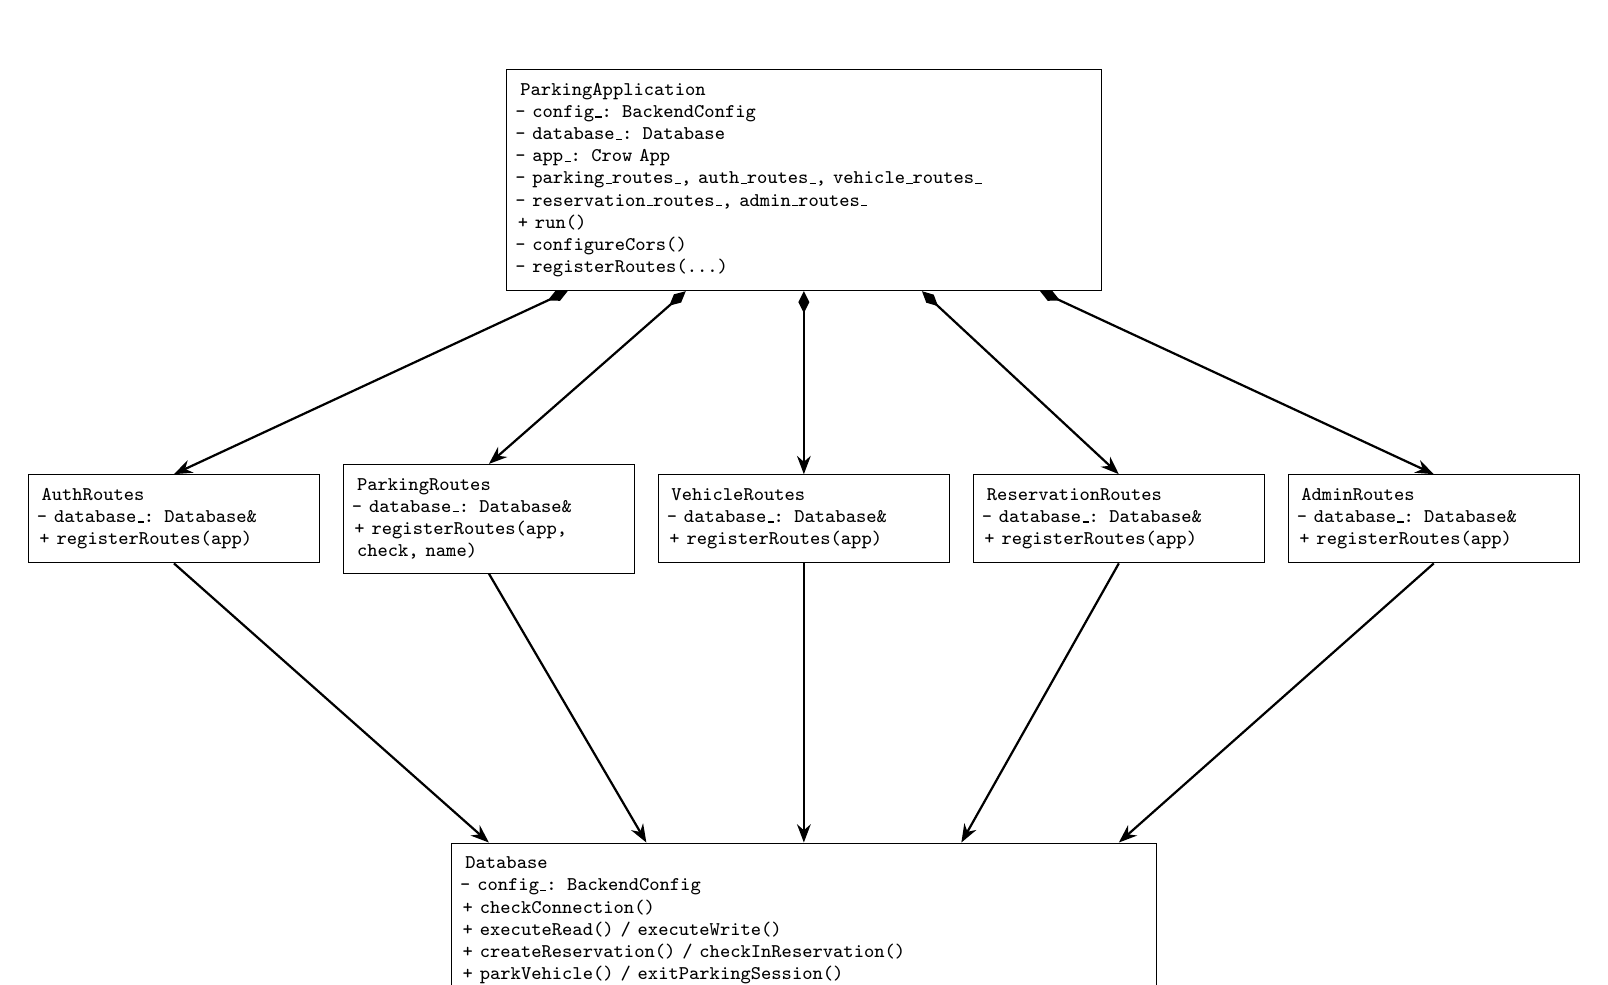
\begin{tikzpicture}[
  classbox/.style={draw,rectangle,align=left,text width=3.35cm,inner sep=5pt,font=\scriptsize\ttfamily},
  compose/.style={{Diamond[fill=black]}-{Stealth},thick},
  assoc/.style={-{Stealth},thick}
]
\node[classbox,text width=7.2cm] (app) at (0,6.0) {\textbf{ParkingApplication}\\
- config\_: BackendConfig\\- database\_: Database\\- app\_: Crow App\\
- parking\_routes\_, auth\_routes\_, vehicle\_routes\_\\
- reservation\_routes\_, admin\_routes\_\\
+ run()\\- configureCors()\\- registerRoutes(...)};
\node[classbox] (auth) at (-8,1.7) {\textbf{AuthRoutes}\\
- database\_: Database\&\\+ registerRoutes(app)};
\node[classbox] (park) at (-4,1.7) {\textbf{ParkingRoutes}\\
- database\_: Database\&\\+ registerRoutes(app, check, name)};
\node[classbox] (vehicle) at (0,1.7) {\textbf{VehicleRoutes}\\
- database\_: Database\&\\+ registerRoutes(app)};
\node[classbox] (reserve) at (4,1.7) {\textbf{ReservationRoutes}\\
- database\_: Database\&\\+ registerRoutes(app)};
\node[classbox] (admin) at (8,1.7) {\textbf{AdminRoutes}\\
- database\_: Database\&\\+ registerRoutes(app)};
\node[classbox,text width=8.6cm] (db) at (0,-3.4) {\textbf{Database}\\
- config\_: BackendConfig\\
+ checkConnection()\\+ executeRead() / executeWrite()\\
+ createReservation() / checkInReservation()\\
+ parkVehicle() / exitParkingSession()};
% Separate source and target points keep each relationship distinguishable.
\draw[compose] ([xshift=-3.0cm]app.south) -- (auth.north);
\draw[compose] ([xshift=-1.5cm]app.south) -- (park.north);
\draw[compose] (app.south) -- (vehicle.north);
\draw[compose] ([xshift=1.5cm]app.south) -- (reserve.north);
\draw[compose] ([xshift=3.0cm]app.south) -- (admin.north);
% Each controller has its own association endpoint on the shared Database.
\draw[assoc] (auth.south) -- ([xshift=-4.0cm]db.north);
\draw[assoc] (park.south) -- ([xshift=-2.0cm]db.north);
\draw[assoc] (vehicle.south) -- (db.north);
\draw[assoc] (reserve.south) -- ([xshift=2.0cm]db.north);
\draw[assoc] (admin.south) -- ([xshift=4.0cm]db.north);
\end{tikzpicture}%
}
\caption{UML class diagram of the custom C++ application structure.}
\label{fig:class}
\end{figure}

The nine implemented concepts are summarized in Table~\ref{tab:oop-concepts}
and demonstrated in Listings~\ref{lst:controller-class}--\ref{lst:raii-exceptions}.
The project does not use a custom inheritance hierarchy or runtime
polymorphism. Records such as users and vehicles are represented by SQL rows
and JSON rather than custom C++ domain entity classes.

\subsection{Architecture}
Figure~\ref{fig:architecture} shows the implemented request path. The browser
uses the JSON API; Crow route controllers validate and authorize requests;
the database layer performs reads and transactional writes against PostgreSQL.

\begin{figure}[H]
\centering
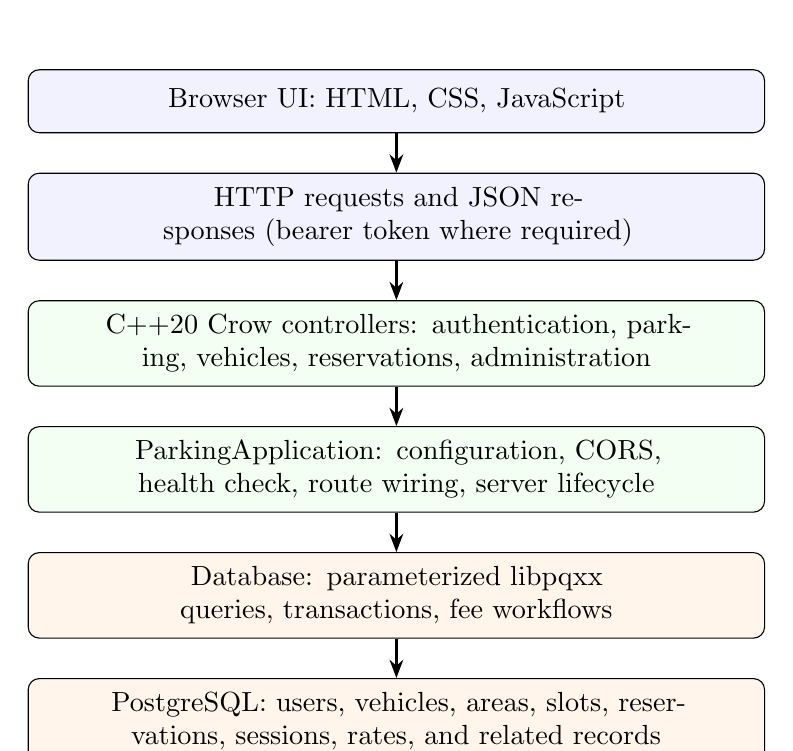
\begin{tikzpicture}[
  layer/.style={draw,rounded corners,align=center,text width=9cm,minimum height=0.8cm,inner sep=5pt},
  flow/.style={-{Stealth},thick},node distance=5mm
]
\node[layer,fill=blue!5] (web) {Browser UI: HTML, CSS, JavaScript};
\node[layer,fill=blue!5,below=of web] (http) {HTTP requests and JSON responses (bearer token where required)};
\node[layer,fill=green!5,below=of http] (routes) {C++20 Crow controllers: authentication, parking, vehicles, reservations, administration};
\node[layer,fill=green!5,below=of routes] (app) {ParkingApplication: configuration, CORS, health check, route wiring, server lifecycle};
\node[layer,fill=orange!8,below=of app] (db) {Database: parameterized libpqxx queries, transactions, fee workflows};
\node[layer,fill=orange!8,below=of db] (pg) {PostgreSQL: users, vehicles, areas, slots, reservations, sessions, rates, and related records};
\draw[flow] (web)--(http); \draw[flow] (http)--(routes); \draw[flow] (routes)--(app); \draw[flow] (app)--(db); \draw[flow] (db)--(pg);
\end{tikzpicture}
\caption{Implemented system architecture and request path.}
\label{fig:architecture}
\end{figure}

\subsection{Reservation Sequence Diagram}
Figure~\ref{fig:sequence} shows the principal reservation workflow. The route
checks the authenticated identity and request data, then delegates the
consistency-sensitive work to the database transaction. The database checks
the vehicle, slot, time range, and conflicts before committing the reservation.

\begin{figure}[H]
\centering
\resizebox{\textwidth}{!}{%
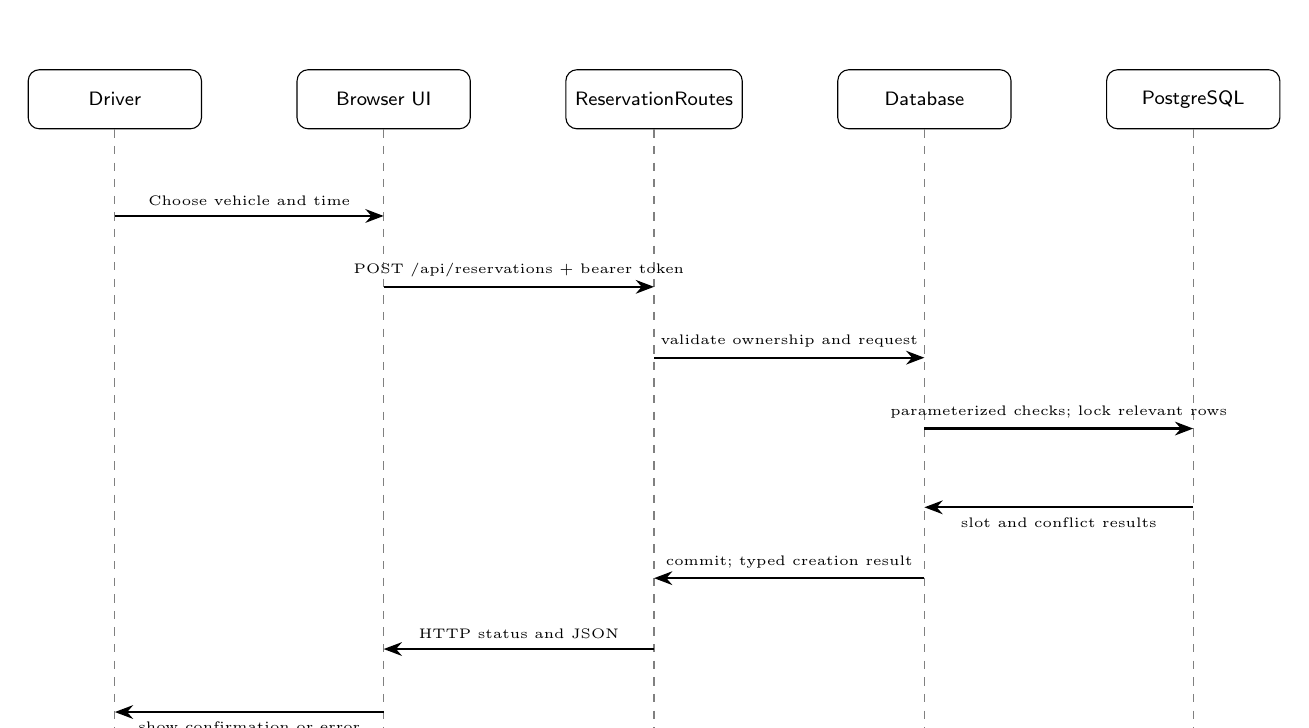
\begin{tikzpicture}[
  actor/.style={draw,rounded corners,minimum width=2.2cm,minimum height=0.75cm,align=center,font=\scriptsize\sffamily},
  msg/.style={-{Stealth},thick},
  lifeline/.style={dashed,gray},
  node distance=1.2cm
]
\node[actor] (user) {Driver};
\node[actor,right=of user] (browser) {Browser UI};
\node[actor,right=of browser] (route) {ReservationRoutes};
\node[actor,right=of route] (db) {Database};
\node[actor,right=of db] (pg) {PostgreSQL};
\foreach \n in {user,browser,route,db,pg} \draw[lifeline] (\n.south) -- ++(0,-7.7);
\draw[msg] ([yshift=-1.1cm]user.south) -- node[above,font=\tiny]{Choose vehicle and time} ([yshift=-1.1cm]browser.south);
\draw[msg] ([yshift=-2.0cm]browser.south) -- node[above,font=\tiny]{POST /api/reservations + bearer token} ([yshift=-2.0cm]route.south);
\draw[msg] ([yshift=-2.9cm]route.south) -- node[above,font=\tiny]{validate ownership and request} ([yshift=-2.9cm]db.south);
\draw[msg] ([yshift=-3.8cm]db.south) -- node[above,font=\tiny]{parameterized checks; lock relevant rows} ([yshift=-3.8cm]pg.south);
\draw[msg] ([yshift=-4.8cm]pg.south) -- node[below,font=\tiny]{slot and conflict results} ([yshift=-4.8cm]db.south);
\draw[msg] ([yshift=-5.7cm]db.south) -- node[above,font=\tiny]{commit; typed creation result} ([yshift=-5.7cm]route.south);
\draw[msg] ([yshift=-6.6cm]route.south) -- node[above,font=\tiny]{HTTP status and JSON} ([yshift=-6.6cm]browser.south);
\draw[msg] ([yshift=-7.4cm]browser.south) -- node[below,font=\tiny]{show confirmation or error} ([yshift=-7.4cm]user.south);
\end{tikzpicture}%
}
\caption{Sequence diagram for reservation creation.}
\label{fig:sequence}
\end{figure}

\subsection{Activity Diagram: Direct Parking}
Figure~\ref{fig:activity} describes direct parking at a compatible slot. The
transaction locks the vehicle and slot, checks ownership and eligibility,
rejects conflicts, updates slot state, creates the assignment, and commits.

\begin{figure}[H]
\centering
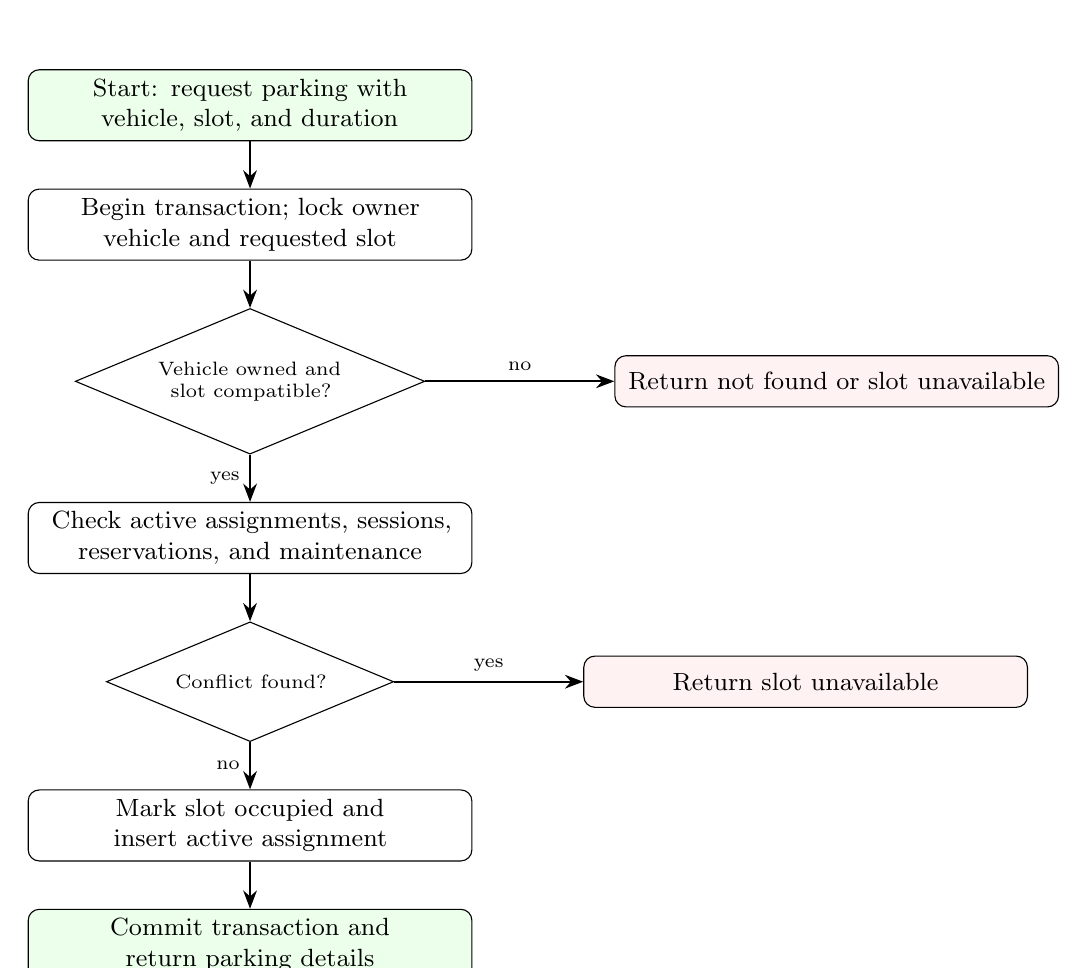
\begin{tikzpicture}[
  activitybox/.style={draw,rounded corners,align=center,text width=5.4cm,minimum height=0.65cm,font=\small},
  decision/.style={draw,diamond,aspect=2.4,align=center,inner sep=1pt,text width=3cm,font=\scriptsize},
  flow/.style={-{Stealth},thick},node distance=6mm
]
\node[activitybox,fill=green!8] (start) {Start: request parking with vehicle, slot, and duration};
\node[activitybox,below=of start] (lock) {Begin transaction; lock owner vehicle and requested slot};
\node[decision,below=of lock] (valid) {Vehicle owned and slot compatible?};
\node[activitybox,below=of valid] (conflict) {Check active assignments, sessions, reservations, and maintenance};
\node[decision,below=of conflict] (free) {Conflict found?};
\node[activitybox,below=of free] (write) {Mark slot occupied and insert active assignment};
\node[activitybox,below=of write,fill=green!8] (commit) {Commit transaction and return parking details};
\node[activitybox,right=2.4cm of valid,fill=red!5] (reject1) {Return not found or slot unavailable};
\node[activitybox,right=2.4cm of free,fill=red!5] (reject2) {Return slot unavailable};
\draw[flow] (start)--(lock); \draw[flow] (lock)--(valid);
\draw[flow] (valid)--node[left,font=\scriptsize]{yes}(conflict);
\draw[flow] (valid.east)--node[above,font=\scriptsize]{no}(reject1.west);
\draw[flow] (conflict)--(free);
\draw[flow] (free)--node[left,font=\scriptsize]{no}(write);
\draw[flow] (free.east)--node[above,font=\scriptsize]{yes}(reject2.west);
\draw[flow] (write)--(commit);
\end{tikzpicture}
\caption{Activity diagram for a direct parking assignment.}
\label{fig:activity}
\end{figure}

\subsection{Use Case Diagram}
Figure~\ref{fig:usecase} summarizes user-facing capabilities. The administrator
inherits the ordinary authenticated-user capabilities and adds management
operations; the diagram uses generalization for actor roles, not for C++
classes.

\begin{figure}[H]
\centering
\resizebox{0.96\textwidth}{!}{%
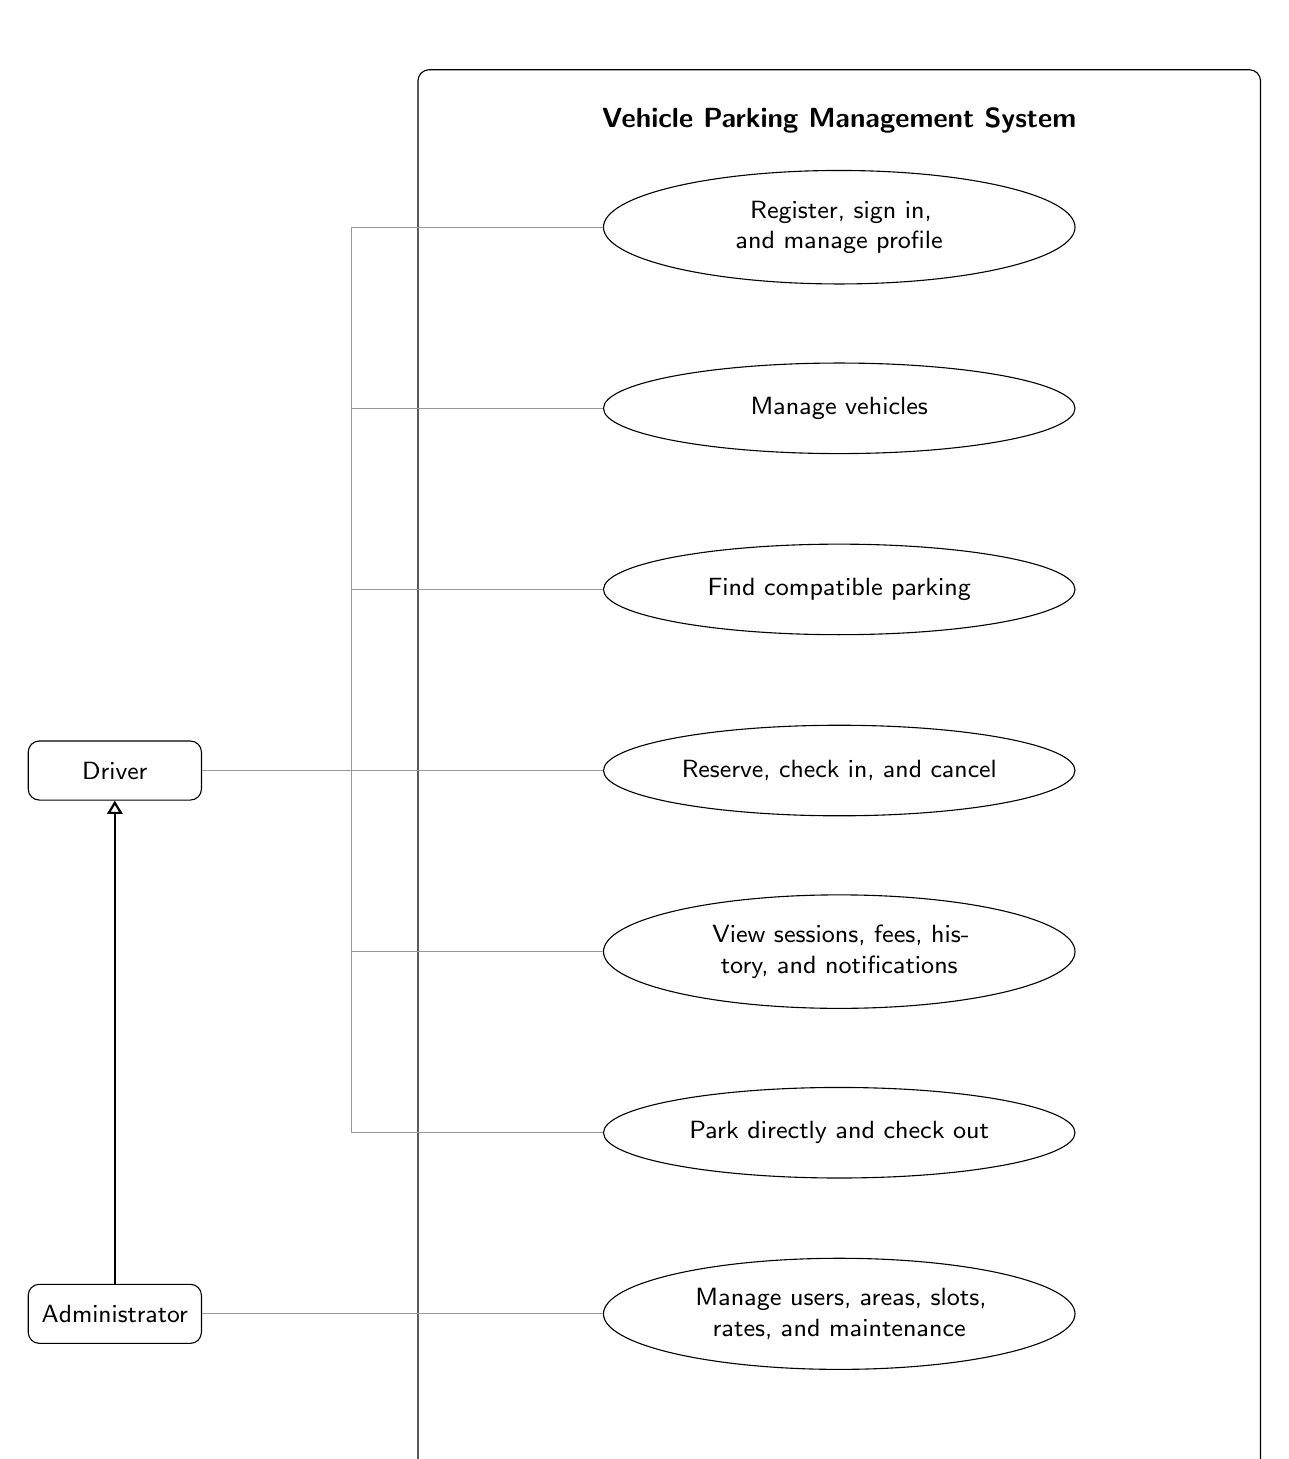
\begin{tikzpicture}[
  actor/.style={draw,rounded corners,align=center,minimum width=2.2cm,minimum height=0.75cm,font=\small\sffamily},
  usecase/.style={draw,ellipse,align=center,text width=4cm,minimum height=1.15cm,inner ysep=5pt,font=\small\sffamily},
  link/.style={draw,gray!80},
  include/.style={-{Stealth},dashed,gray!70},
  generalize/.style={-{Triangle[open]},thick}
]
\node[draw,rounded corners,minimum width=10.7cm,minimum height=17.8cm] (boundary) at (2,-0.5) {};
\node[font=\bfseries\sffamily] at (2,7.75) {Vehicle Parking Management System};
\node[actor] (driver) at (-7.2,-0.5) {Driver};
\node[actor] (admin) at (-7.2,-7.4) {Administrator};
\node[usecase] (account) at (2,6.4) {Register, sign in, and manage profile};
\node[usecase] (vehicles) at (2,4.1) {Manage vehicles};
\node[usecase] (availability) at (2,1.8) {Find compatible parking};
\node[usecase] (reserve) at (2,-0.5) {Reserve, check in, and cancel};
\node[usecase] (sessions) at (2,-2.8) {View sessions, fees, history, and notifications};
\node[usecase] (direct) at (2,-5.1) {Park directly and check out};
\node[usecase] (manage) at (2,-7.4) {Manage users, areas, slots, rates, and maintenance};
% Route driver links outside the use cases so no line crosses an oval.
\coordinate (driverbus) at (-4.2,-0.5);
\draw[link] (driver.east)--(driverbus);
\draw[link] (-4.2,6.4)--(-4.2,-5.1);
\foreach \n in {account,vehicles,availability,reserve,sessions,direct} {
  \draw[link] (driverbus |- \n.west) -- (\n.west);
}
\draw[link] (admin.east)--(manage.west);
\draw[generalize] (admin.north) -- (driver.south);
\end{tikzpicture}%
}
\caption{Use case diagram for driver and administrator roles.}
\label{fig:usecase}
\end{figure}

\subsection{OOP Code Examples}
Listing~\ref{lst:controller-class} shows a project class declaration. The
private \texttt{database\_} reference demonstrates encapsulation and its
association with the shared \texttt{Database} object.

\begin{lstlisting}[caption={AuthRoutes class declaration: public operations and private associated database.},label={lst:controller-class}]
class AuthRoutes
{
public:
    explicit AuthRoutes(Database &database);
    void registerRoutes(crow::App<crow::CORSHandler> &app);

private:
    Database &database_;
};
\end{lstlisting}

Listing~\ref{lst:composition} is taken from the implemented application
constructor. It demonstrates composition: the application owns its database
and controller members, and injects the shared database by reference into each
controller.

\begin{lstlisting}[caption={Implemented dependency wiring in ParkingApplication.},label={lst:composition}]
ParkingApplication::ParkingApplication(const BackendConfig &config)
    : config_(config),
      database_(config_),
      parking_routes_(database_),
      auth_routes_(database_),
      vehicle_routes_(database_),
      reservation_routes_(database_),
      admin_routes_(database_)
{
}
\end{lstlisting}

The same construction pattern demonstrates constructors and dependency
injection: \texttt{ParkingApplication} passes its already-created database to
the controllers. The application object itself is constructed in
\texttt{main()} and its public \texttt{run()} method hides startup details.

\begin{lstlisting}[caption={Application startup orchestration behind the run() abstraction.},label={lst:run-abstraction}]
void ParkingApplication::run()
{
    configureCors();

    const DatabaseCheckResult database_check = database_.checkConnection();
    if (database_check.connected)
    {
        std::cout << "Database check successful!" << std::endl;
    }
    else
    {
        std::cerr << "Database connection failed: "
                  << database_check.error_message << std::endl;
    }

    registerRoutes(database_check);

    std::cout << "Server running on http://localhost:"
              << config_.server_port << std::endl;
    app_.port(config_.server_port).multithreaded().run();
}
\end{lstlisting}

Listing~\ref{lst:fees} is the project's fee calculation value type and function.
It shows a small, cohesive abstraction with an explicit result structure,
nonnegative overtime handling, whole-hour booking billing, and currency
rounding.

\begin{lstlisting}[caption={Implemented fee calculation in parking\_fees.h.},label={lst:fees}]
struct Breakdown
{
    int billed_hours;
    int billed_overtime_minutes;
    double base_fee;
    double overtime_fee;
    double total_fee;
};

inline Breakdown calculate(
    int booked_duration_minutes,
    int overtime_duration_seconds,
    double hourly_rate)
{
    const int billed_hours = std::max(1, (booked_duration_minutes + 59) / 60);
    const int nonnegative_overtime_seconds =
        std::max(0, overtime_duration_seconds);
    const int billed_overtime_minutes = nonnegative_overtime_seconds / 60 +
        (nonnegative_overtime_seconds % 60 != 0 ? 1 : 0);
    const double base_fee = roundCurrency(billed_hours * hourly_rate);
    const double overtime_fee = roundCurrency(
        billed_overtime_minutes * overtime_rate_per_minute);

    return {billed_hours, billed_overtime_minutes, base_fee,
            overtime_fee, roundCurrency(base_fee + overtime_fee)};
}
\end{lstlisting}

The database workflows use \texttt{pqxx::work} transaction objects and
parameterized libpqxx calls. On successful direct parking, the implementation
updates the slot and inserts an assignment before committing.
An early validation return leaves the transaction uncommitted, so transaction
scope handles rollback through RAII. No project class uses custom inheritance
or virtual methods; this describes the current source accurately.

Listing~\ref{lst:raii-exceptions} shows RAII and exception handling together:
the connection and transaction have local lifetimes, and connection failures
are returned as a typed result with an error message.

\begin{lstlisting}[caption={Scoped libpqxx resources and exception handling in the database health check.},label={lst:raii-exceptions}]
DatabaseCheckResult Database::checkConnection() const
{
    try
    {
        pqxx::connection connection = createConnection();
        pqxx::work transaction(connection);
        transaction.exec("SELECT 1");
        transaction.commit();
        return {true, {}};
    }
    catch (const std::exception &exception)
    {
        return {false, exception.what()};
    }
}
\end{lstlisting}

Startup applies the same exception-handling principle: the top-level handler
catches configuration or application failures and exits with an error status.
Route handlers similarly translate database exceptions into HTTP error
responses.

\section{Database Design and Persistence}
The schema in \texttt{database/schema.sql} defines twelve core tables. Identity
records are \texttt{users}, \texttt{auth\_sessions}, and
\texttt{notifications}. Parking resources are \texttt{parking\_areas},
\texttt{parking\_slots}, \texttt{parking\_assignments},
\texttt{parking\_rates}, and \texttt{maintenance}. Reservation and billing
records are \texttt{reservations}, \texttt{parking\_sessions}, and
\texttt{payments}. Primary and foreign keys,
check constraints, unique constraints, and indexes enforce data rules. The
SQL schema and migration scripts are authoritative for database details.

Reservation and parking operations check ownership and conflicts in database
transactions. The schema's partial unique indexes restrict each vehicle and
slot to one active direct parking assignment. Reservations and maintenance
are considered when searching for eligible slots. User-facing CRUD operations
are owner-scoped, while administrator endpoints apply role checks.

\subsection{Fee Rules}
The fee helper bills a minimum of one hour and rounds booked minutes up to whole
hours. Overtime duration is rounded up to whole minutes. The implemented
constants are a seven-minute free buffer and INR 1 per billed overtime minute;
the hourly rate comes from the applicable database rate, with the documented
default of INR 40 where a configured reservation rate is absent. A session's
fee summary includes booked duration, rate, overtime, and total fee.

\section{Project Interface and Execution Outputs}
The frontend source provides a ParkFlow interface with an authentication view,
parking area and slot display, vehicle and reservation workflows, session
history, notifications, and an administrator console. Figures
\ref{fig:auth-screens}--\ref{fig:admin-maintenance} reproduce the browser
screenshots supplied with the project. Each image is stored in the local
\texttt{report\_screenshots/} directory so the report can be compiled without
access to the original OneDrive folder.

\begin{figure}[H]
\centering
\begin{minipage}[t]{0.30\textwidth}\centering
  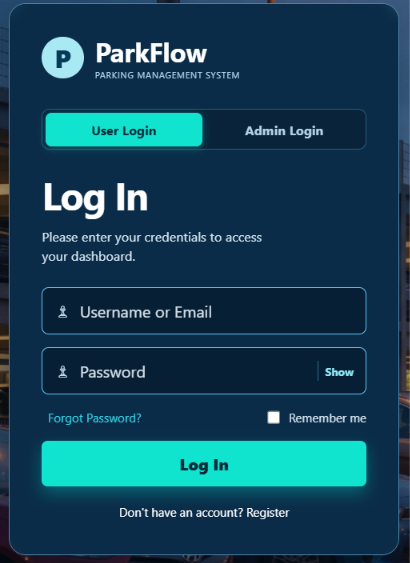
\includegraphics[width=\linewidth,height=0.43\textheight,keepaspectratio]{login.png}\\
  {\small User login}
\end{minipage}\hfill
\begin{minipage}[t]{0.30\textwidth}\centering
  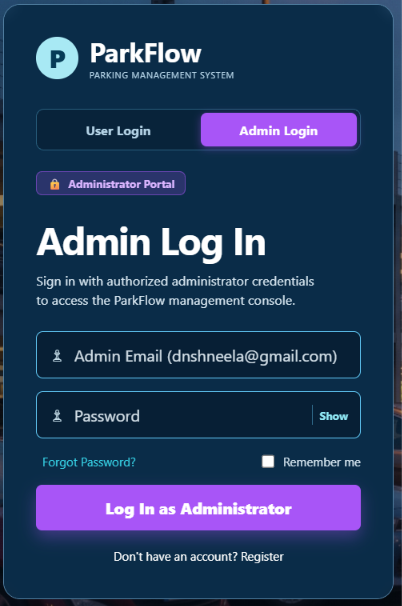
\includegraphics[width=\linewidth,height=0.43\textheight,keepaspectratio]{admin-login.png}\\
  {\small Administrator login}
\end{minipage}\hfill
\begin{minipage}[t]{0.30\textwidth}\centering
  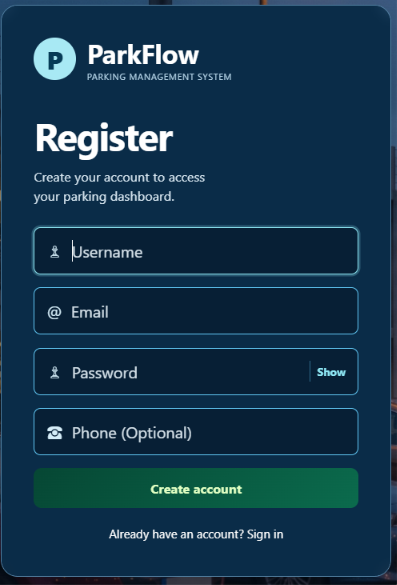
\includegraphics[width=\linewidth,height=0.43\textheight,keepaspectratio]{registration.png}\\
  {\small Account registration}
\end{minipage}
\caption{ParkFlow authentication and registration screens.}
\label{fig:auth-screens}
\end{figure}

\clearpage
\begin{figure}[H]
\centering
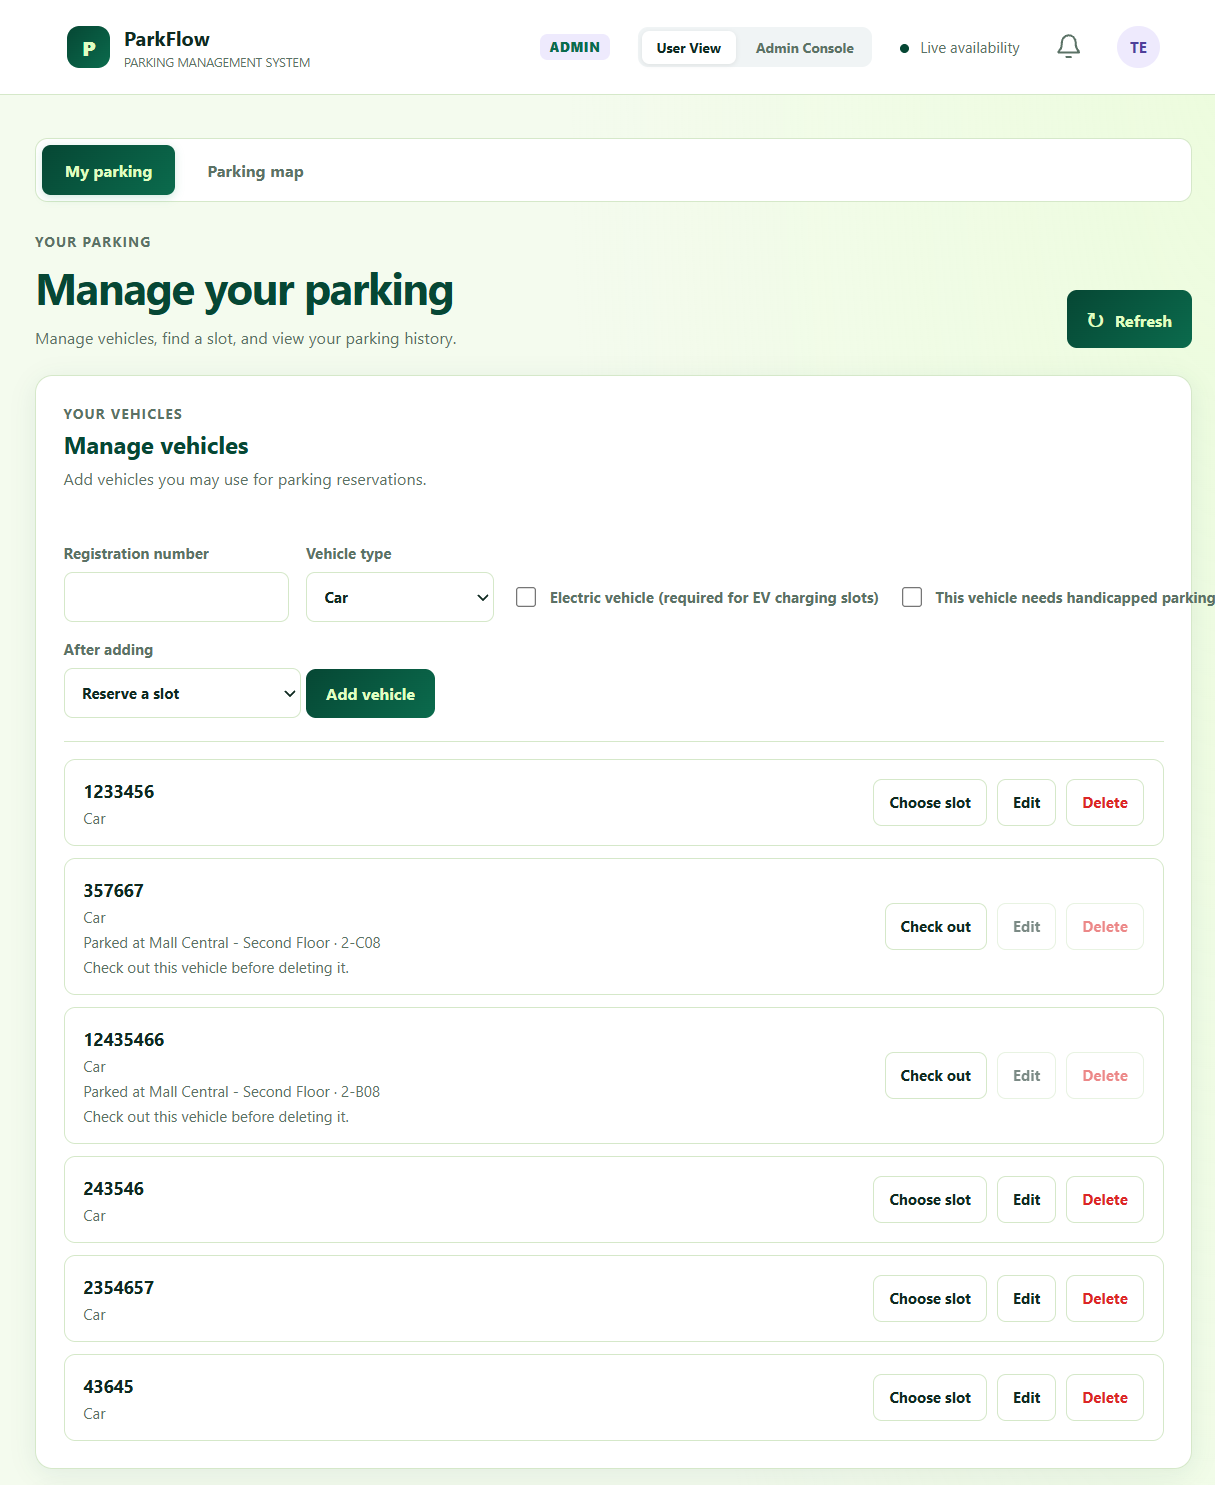
\includegraphics[width=0.97\textwidth]{driver-manage-vehicles.png}
\caption{Driver view: Manage Vehicles.}
\label{fig:driver-manage-vehicles}
\end{figure}
\clearpage
\begin{figure}[H]
\centering
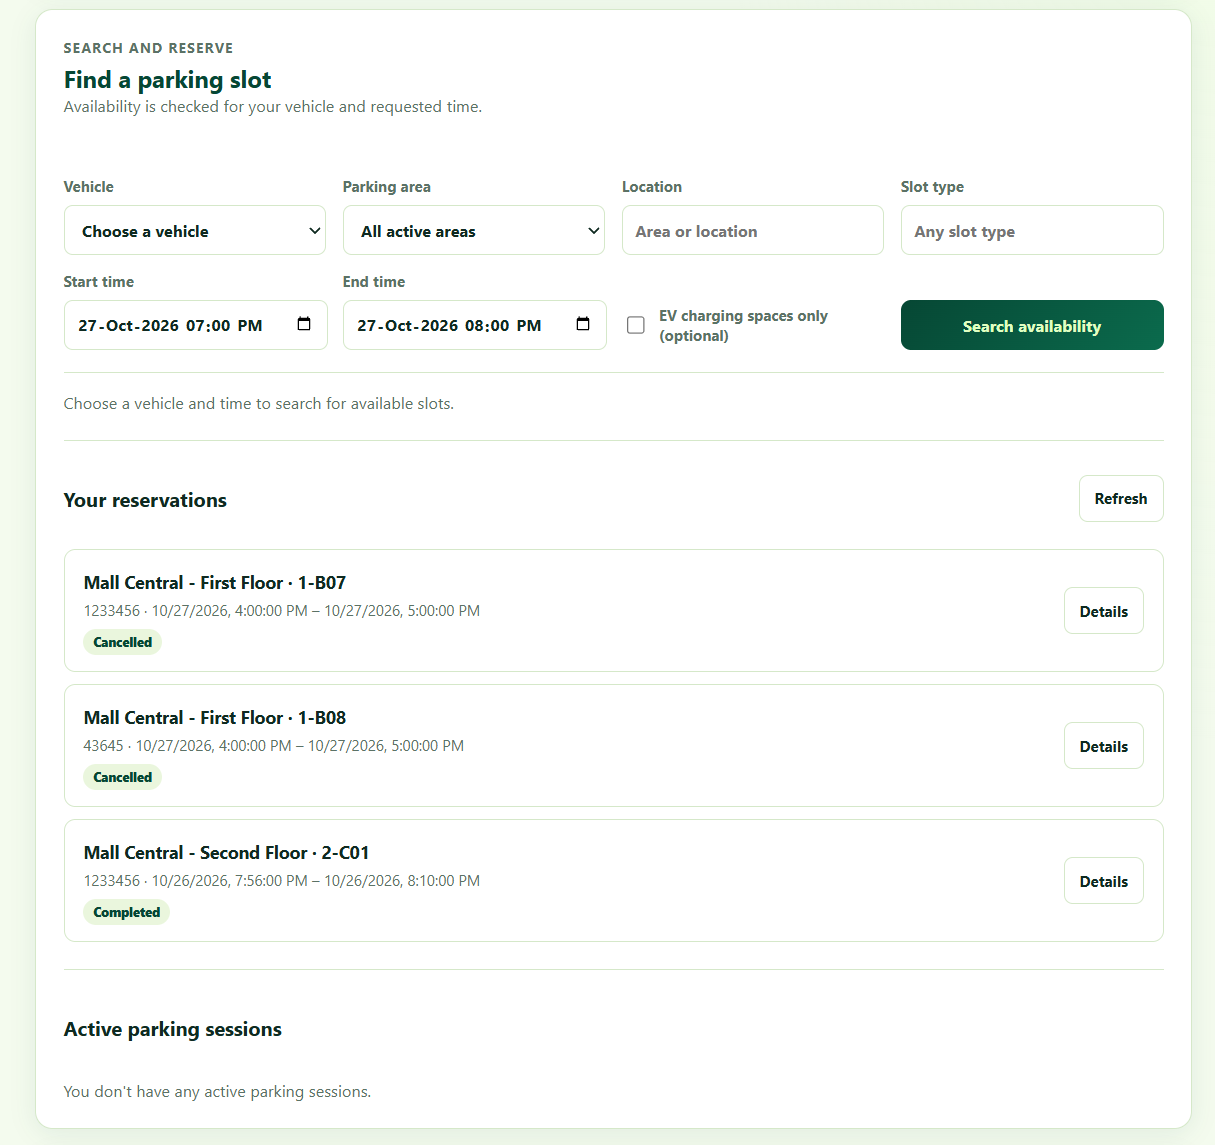
\includegraphics[width=0.97\textwidth]{driver-parking-slot-reservations.png}
\caption{Driver view: Find a Parking Slot, reservations, and active sessions.}
\label{fig:driver-parking-slots}
\end{figure}
\clearpage
\begin{figure}[H]
\centering
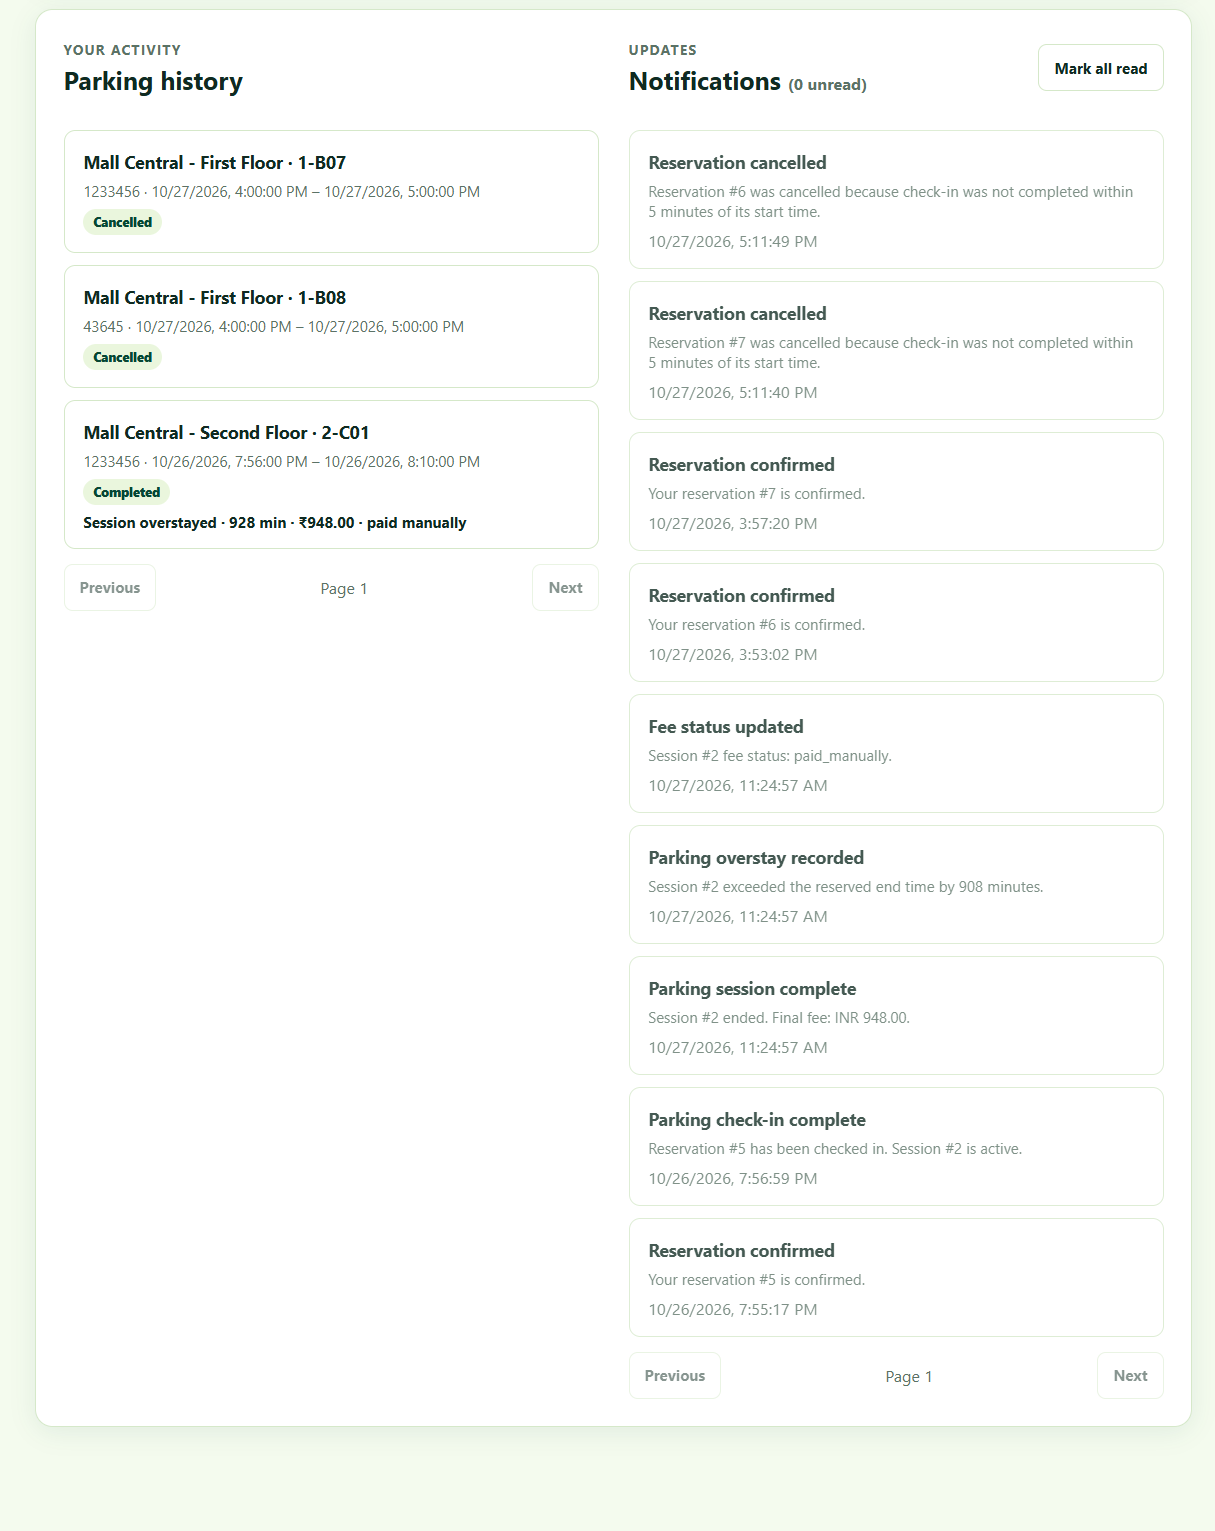
\includegraphics[width=0.97\textwidth]{driver-history-notifications.png}
\caption{Driver view: Parking History and Notifications.}
\label{fig:driver-history-notifications}
\end{figure}
\clearpage

\begin{figure}[H]
\centering
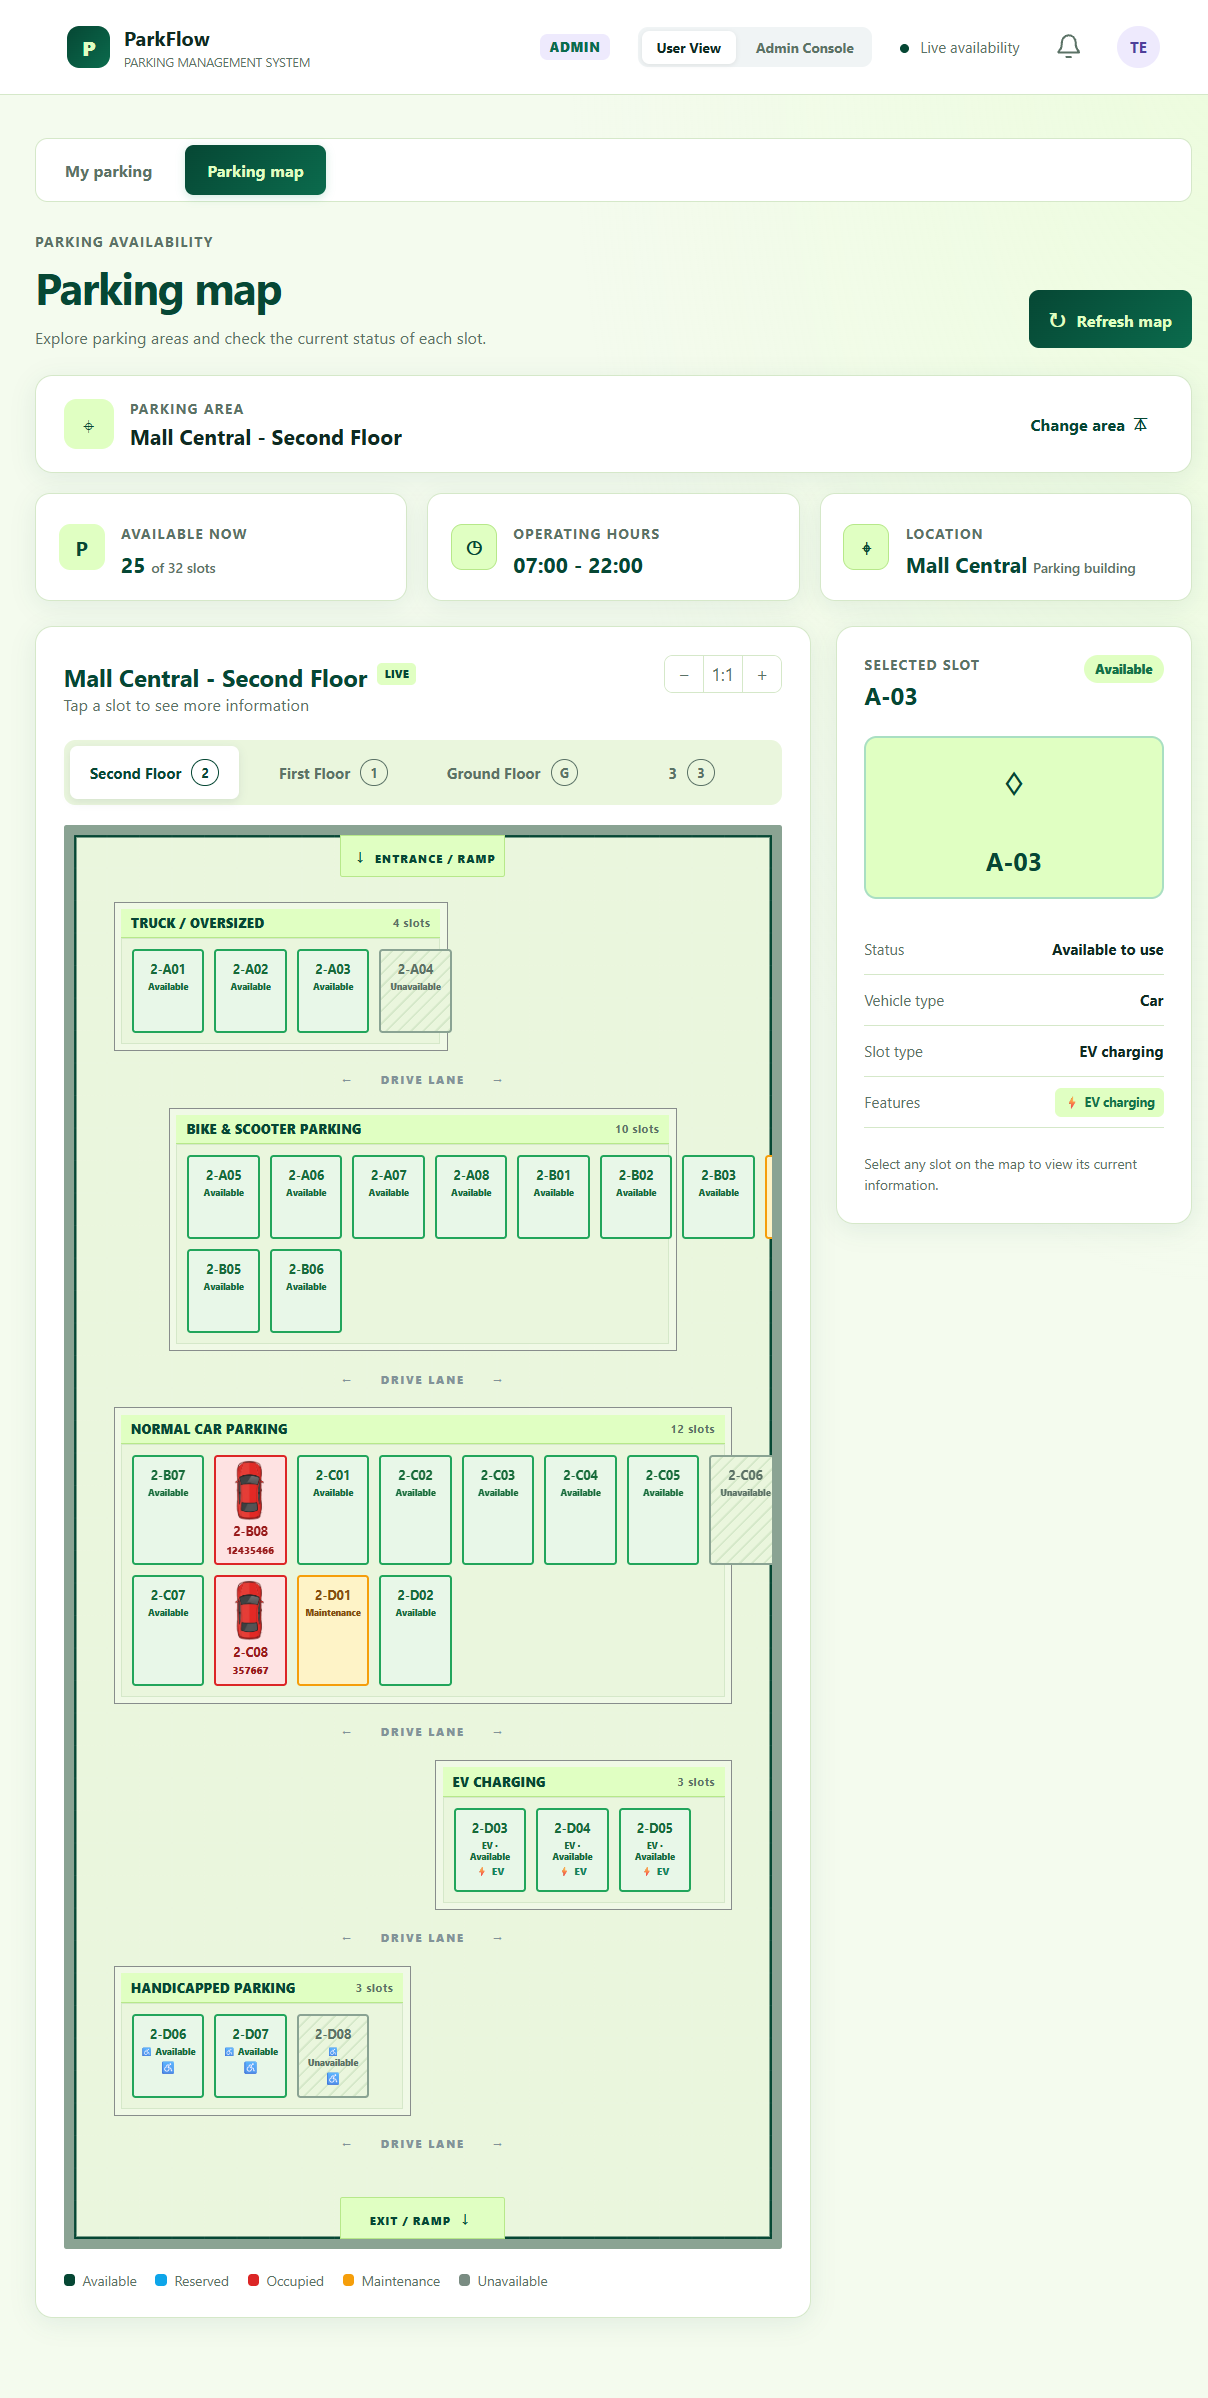
\includegraphics[width=0.80\textwidth,height=0.72\textheight,keepaspectratio]{parking-map.png}
\caption{Parking map with area selection, slot availability, and selected-slot details.}
\label{fig:parking-map}
\end{figure}

\begin{figure}[H]
\centering
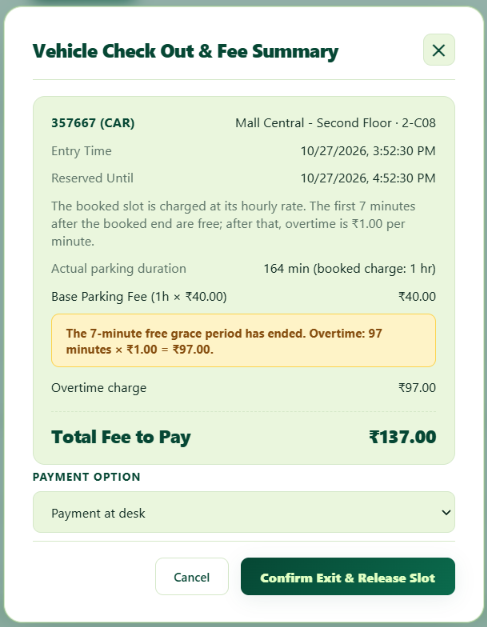
\includegraphics[width=0.72\textwidth,height=0.62\textheight,keepaspectratio]{checkout-fee-summary.png}
\caption{Vehicle checkout fee summary with booked duration, overtime, and payment option.}
\label{fig:checkout-fee}
\end{figure}

\begin{figure}[H]
\centering
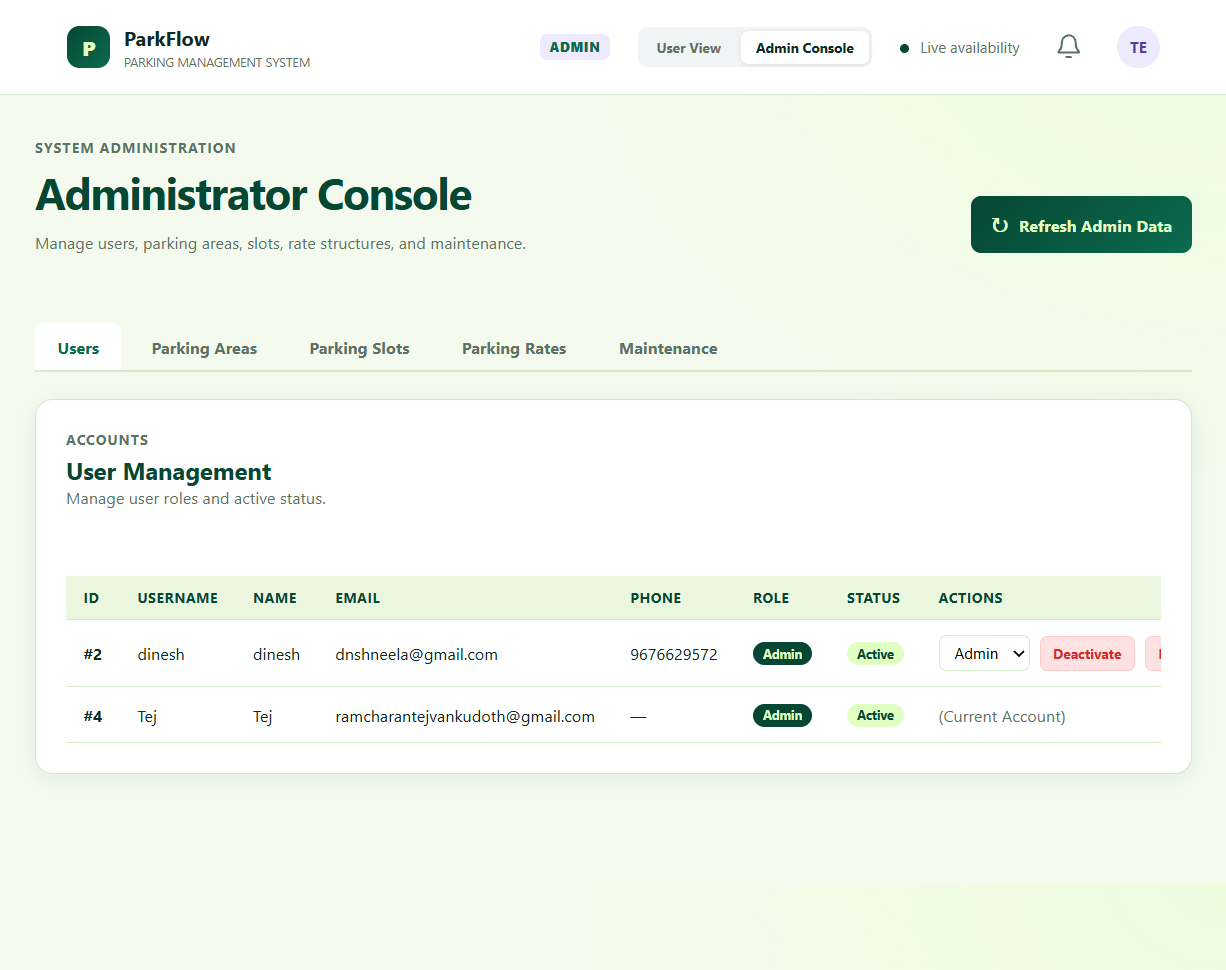
\includegraphics[width=0.92\textwidth,height=0.60\textheight,keepaspectratio]{admin-users.png}
\caption{Administrator user-management screen with role, status, and account actions.}
\label{fig:admin-users}
\end{figure}

\begin{figure}[H]
\centering
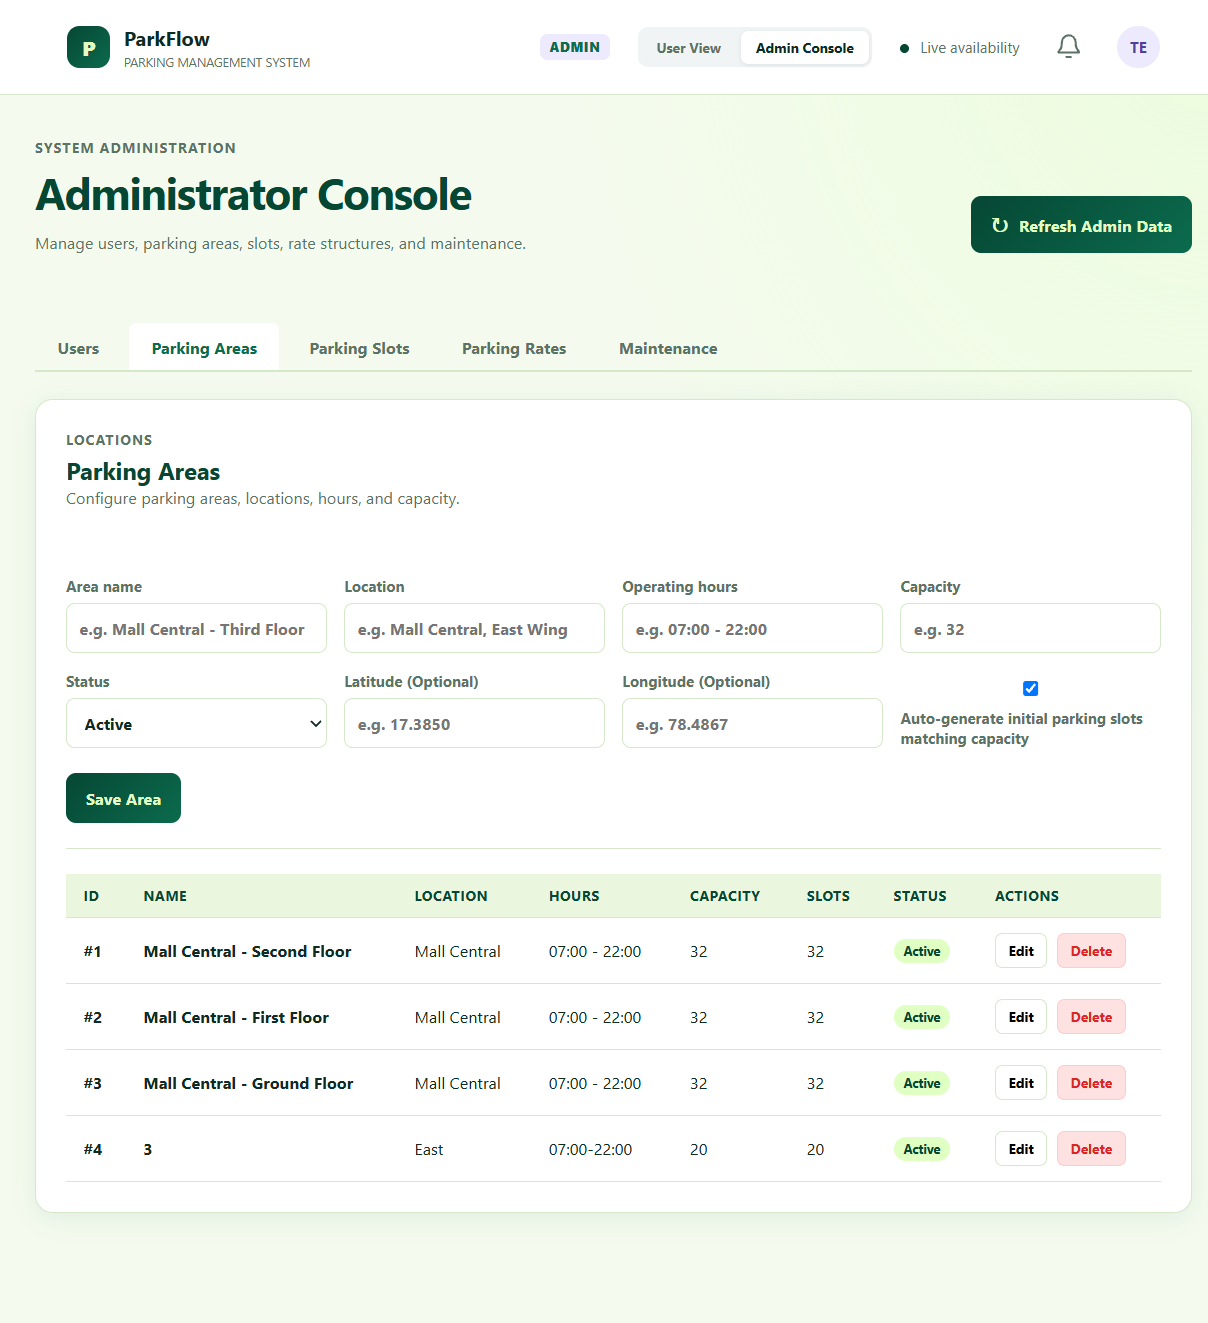
\includegraphics[width=0.85\textwidth,height=0.68\textheight,keepaspectratio]{admin-areas.png}
\caption{Administrator parking-area configuration and area list.}
\label{fig:admin-areas}
\end{figure}

\begin{figure}[H]
\centering
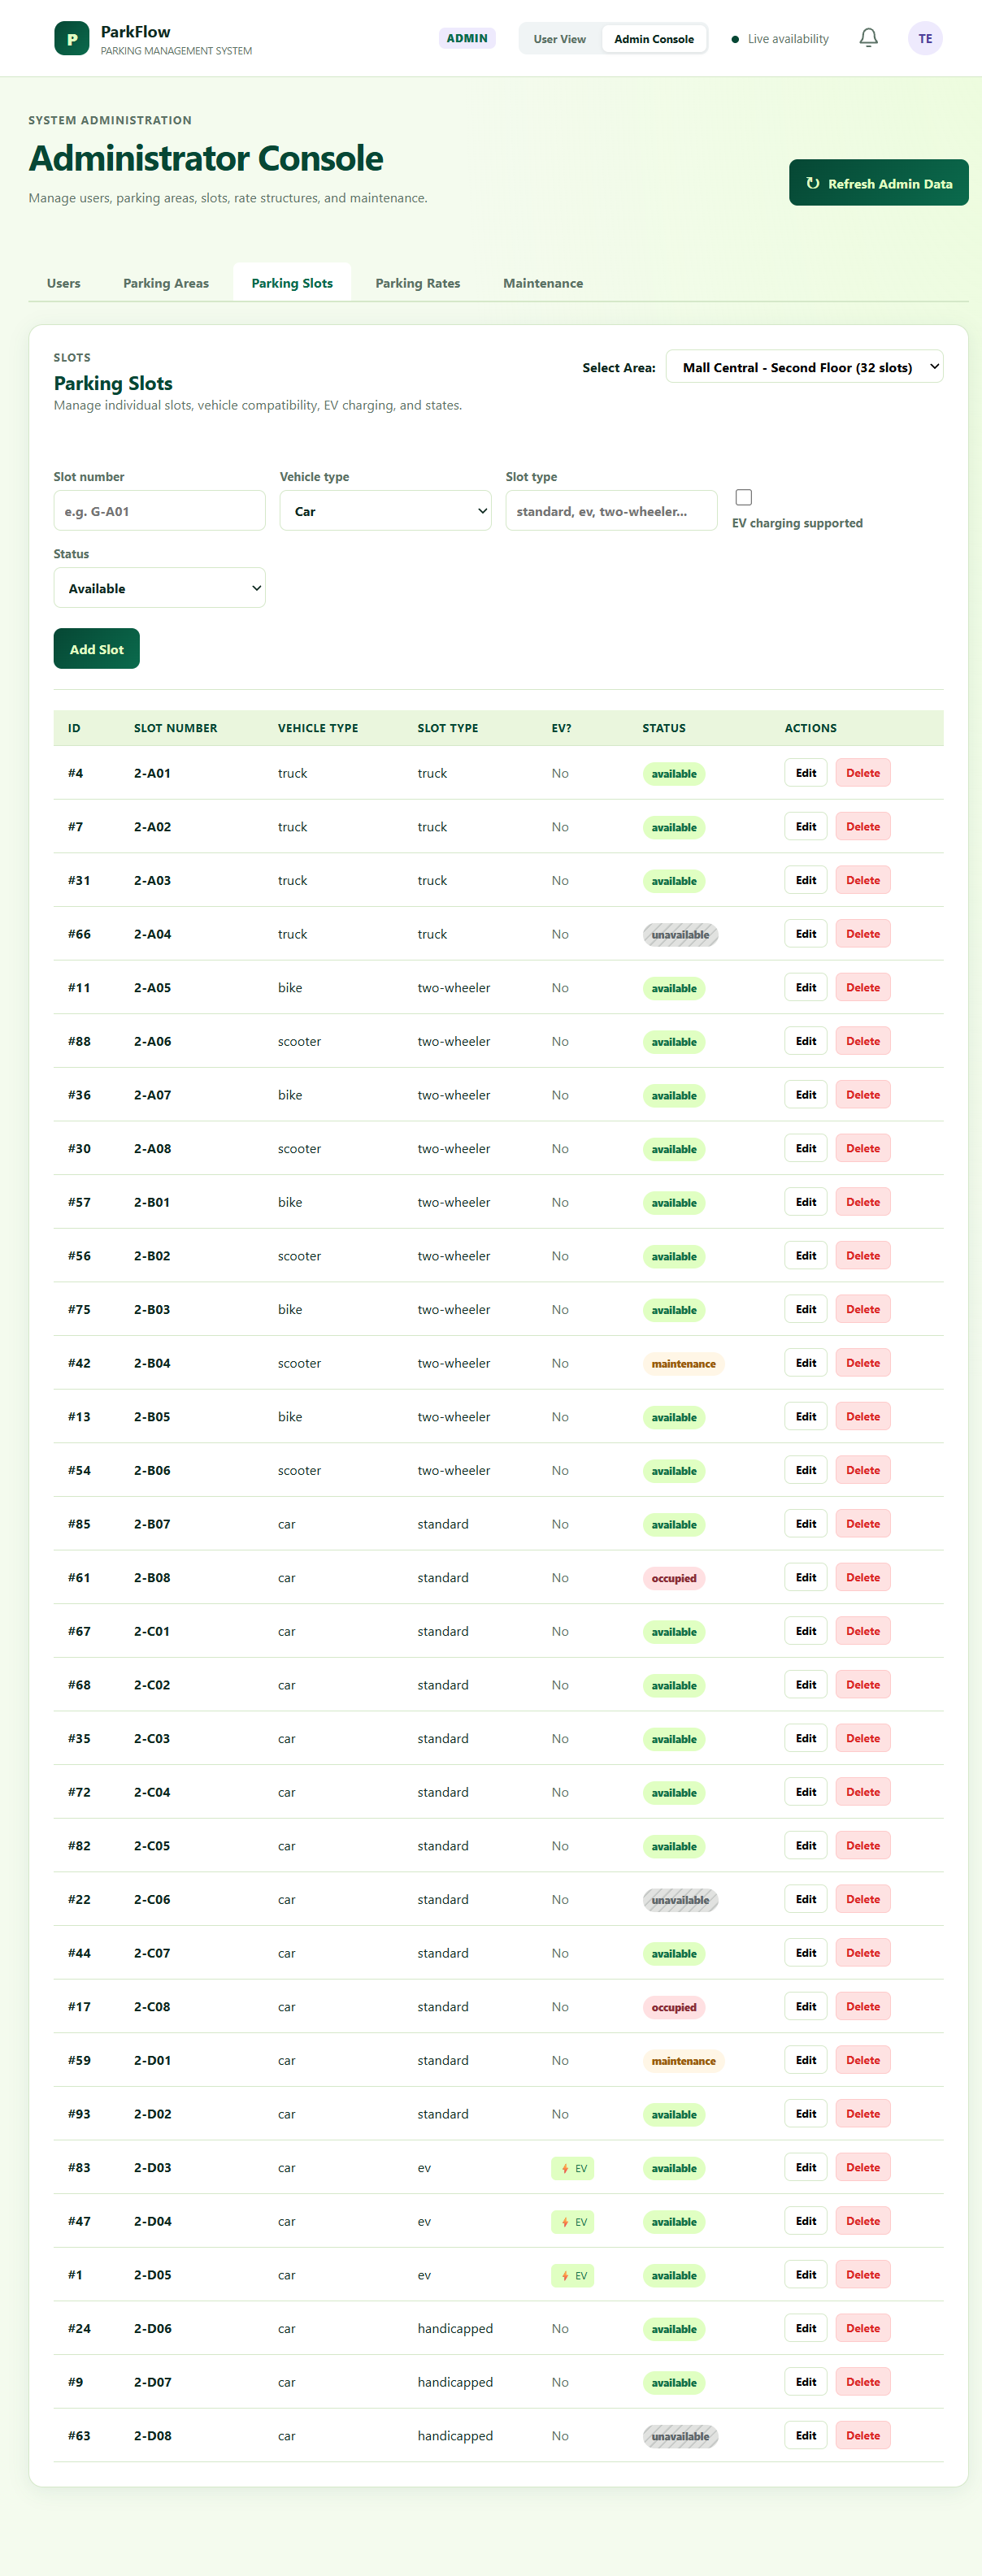
\includegraphics[width=0.82\textwidth,height=0.72\textheight,keepaspectratio]{admin-slots.png}
\caption{Administrator slot configuration and slot inventory.}
\label{fig:admin-slots}
\end{figure}

\begin{figure}[H]
\centering
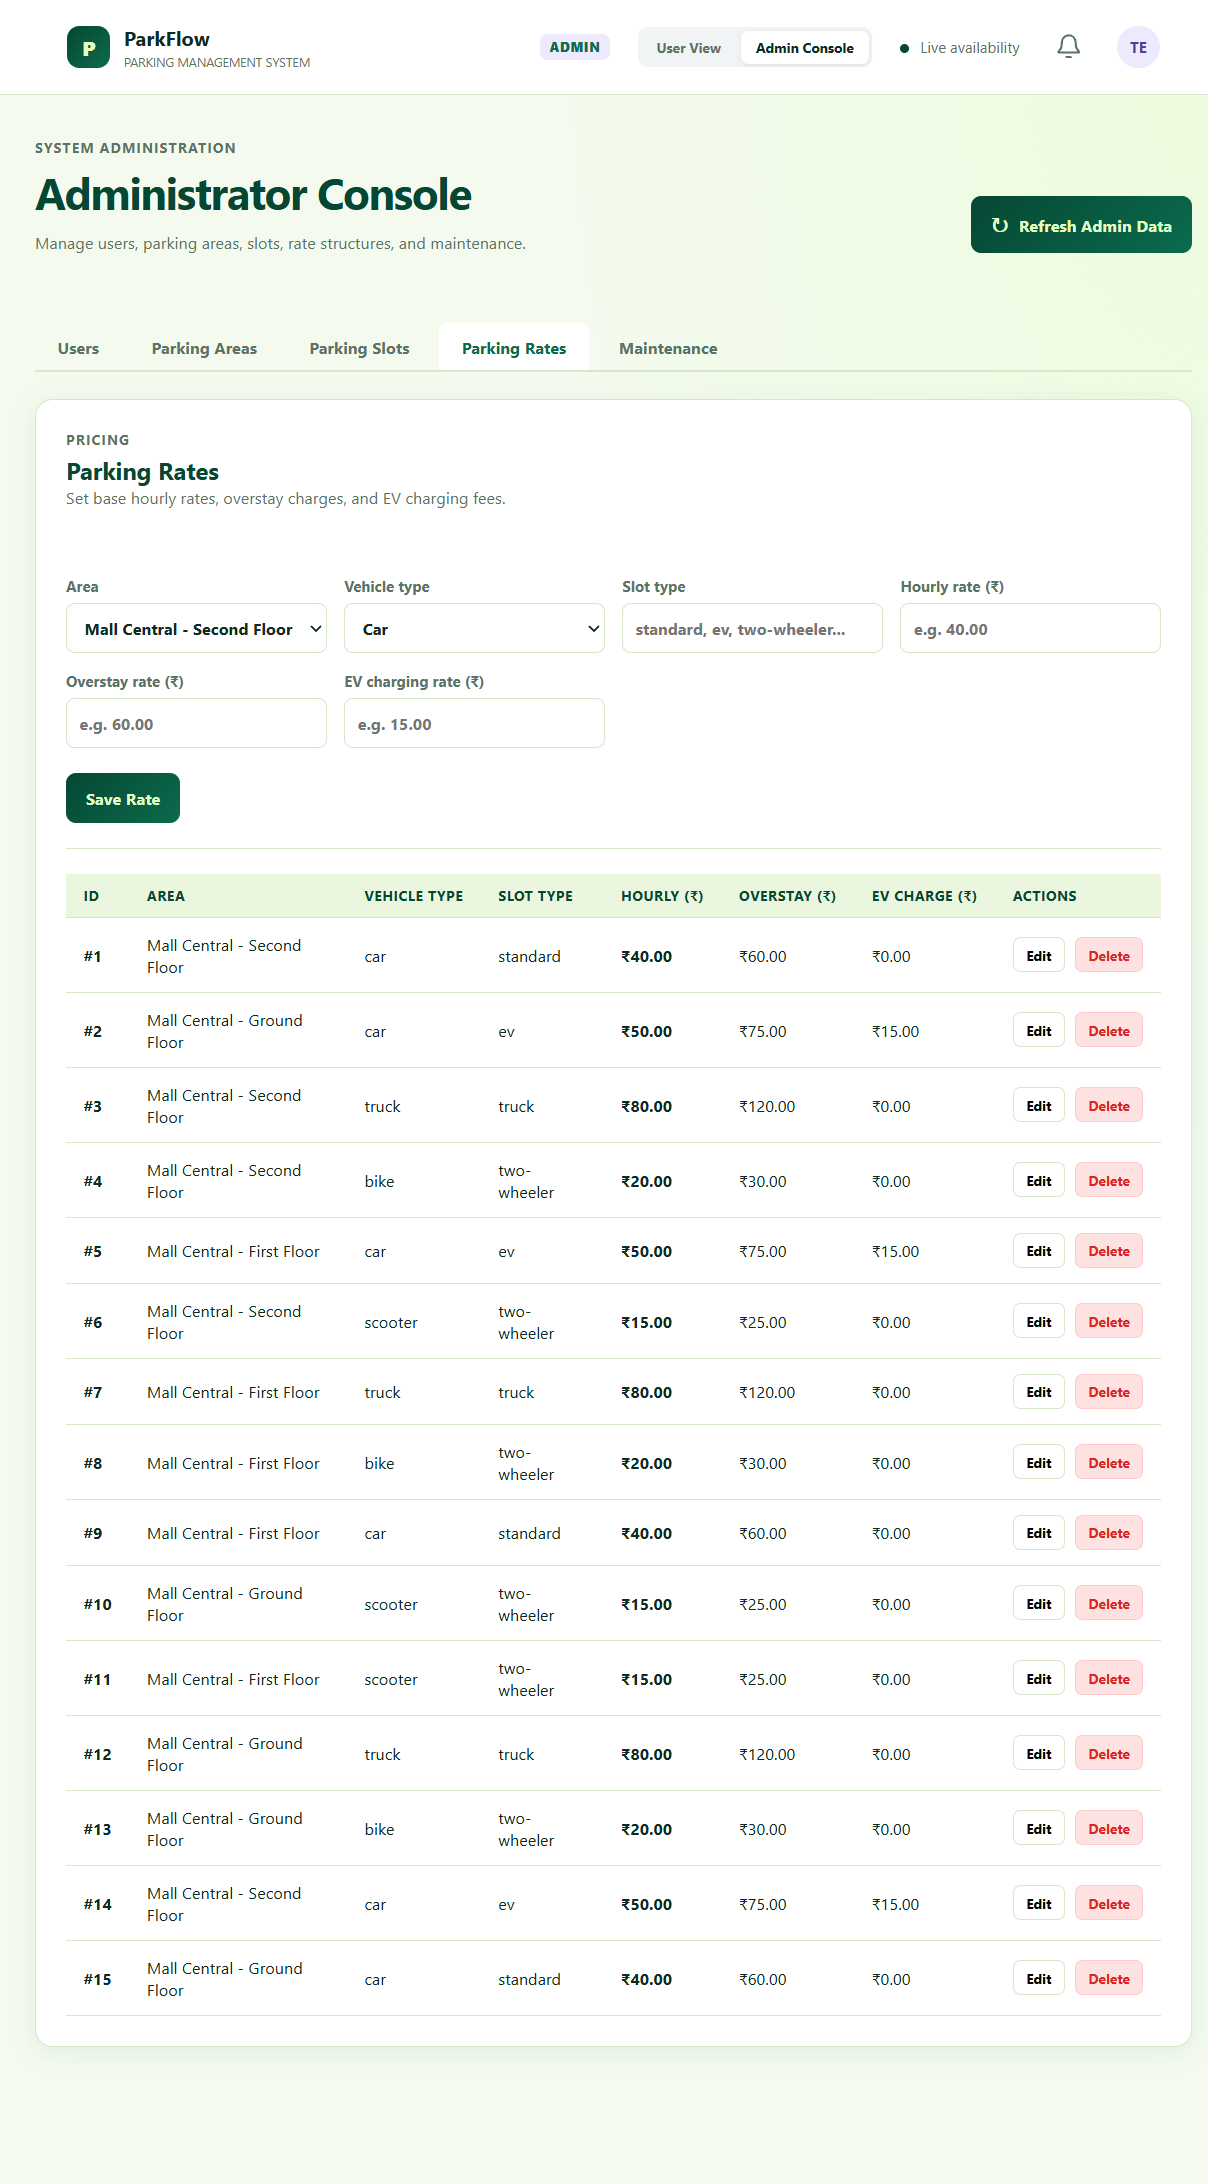
\includegraphics[width=0.82\textwidth,height=0.72\textheight,keepaspectratio]{admin-rates.png}
\caption{Administrator parking-rate configuration and rate list.}
\label{fig:admin-rates}
\end{figure}

\begin{figure}[H]
\centering
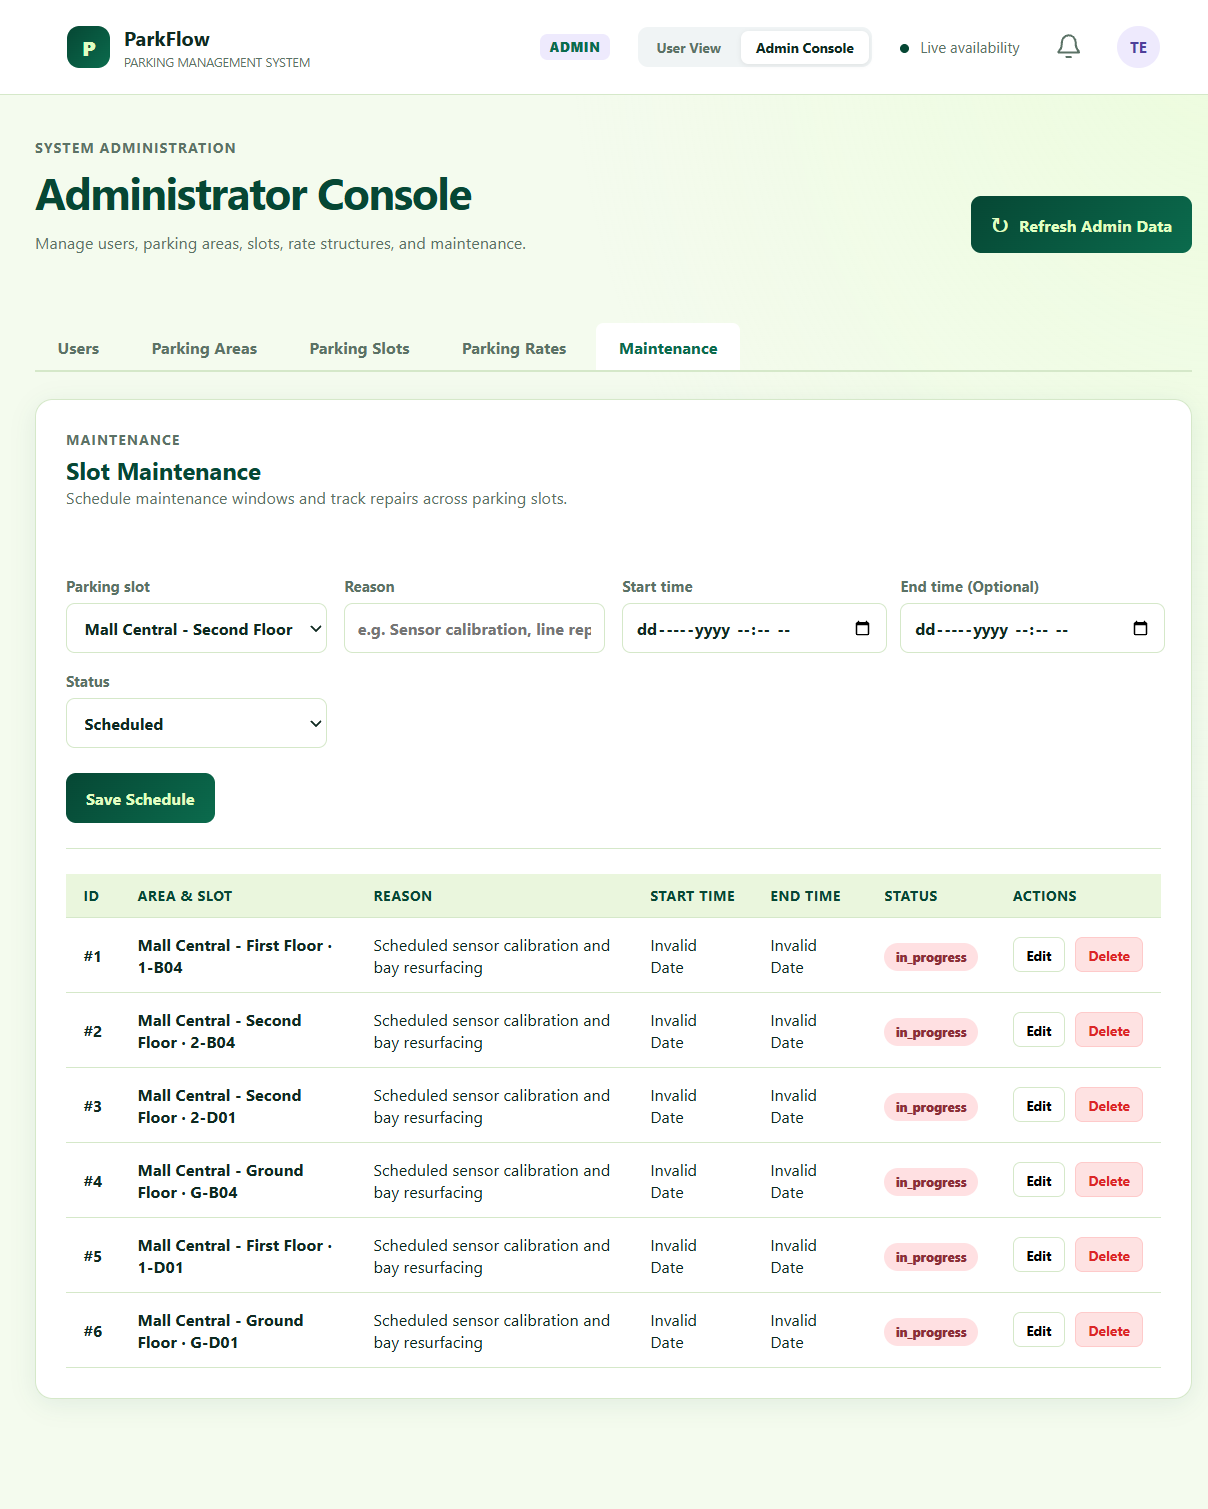
\includegraphics[width=0.85\textwidth,height=0.68\textheight,keepaspectratio]{admin-maintenance.png}
\caption{Administrator maintenance scheduling and maintenance list.}
\label{fig:admin-maintenance}
\end{figure}

\subsection{Build and Run}
The backend build is configured through CMake (minimum version 3.20) and
requires a C++20 compiler, Crow, libpqxx, OpenSSL, and PostgreSQL. The frontend
can be served as static files; it expects the backend at
\texttt{http://localhost:3000} by default. The database password is supplied
through \texttt{PARKING\_DB\_PASSWORD}; secrets should not be included in the
report or committed to source control. Setup and migration commands are
documented in \texttt{README.md}.

\subsection{Project Source Map}
\begin{table}[H]
\centering\small
\begin{tabularx}{\textwidth}{@{}>{\ttfamily\raggedright\arraybackslash}p{2.2in}>{\raggedright\arraybackslash}X@{}}
\toprule
Path & Responsibility \\
\midrule
backend/src/application/ & Application lifecycle, CORS configuration, dependency wiring. \\
backend/src/routes/ & Auth, parking, vehicle, reservation, and administrator HTTP routes. \\
backend/src/database/ & PostgreSQL access, transactions, parking workflows, and fee calculations. \\
backend/src/config/ & Environment-based backend configuration. \\
backend/src/auth/ and validation/ & Password/token functions and request validation helpers. \\
backend/src/api/ & Response value types, JSON serializers, and API errors. \\
frontend/ & HTML interface, styles, JavaScript modules, and image assets. \\
database/ & Schema, migrations, and development seed scripts. \\
\bottomrule
\end{tabularx}
\caption{Source tree responsibilities.}
\label{tab:source-map}
\end{table}

\section{Limitations and Future Work}
The implementation status recorded by the project documentation identifies
automated reservation expiry, QR-based check-in, online payment processing,
refunds, digital receipts, advanced fee rules, external notifications, and
advanced reporting as planned work. The repository also records live Phase 8
database end-to-end verification and production deployment as outstanding.
These items should not be presented as completed functionality.

\section{Conclusion}
VPMS provides a browser-based parking workflow backed by a C++20 Crow API and
PostgreSQL. Its object-oriented structure uses an application composition
root, feature-focused route controllers, and an encapsulated database layer.
Transactional persistence supports reservations, parking assignments,
sessions, billing summaries, history, notifications, and administration. The
design demonstrates practical encapsulation, abstraction, composition, and
RAII while keeping the report aligned with the current implementation.

\end{document}
